% Documents setup
\documentclass[11pt]{book}

% fix for pandoc 1.14
\providecommand{\tightlist}{%
  \setlength{\itemsep}{0pt}\setlength{\parskip}{0pt}}

\usepackage{tabu} % https://tex.stackexchange.com/questions/50332/vertical-spacing-of-a-table-cell

% Location of the csas-style repository: adjust path as needed
\newcommand{\locRepo}{csas-style}

% Use the style file in the csas-style repository (res-doc.sty)
\usepackage{\locRepo/res-doc}

% header-includes from R markdown entry
\usepackage{amsmath}

% Headers and footers
\lhead{Draft working paper --- Do not cite or circulate}
% \lhead{}
\rhead{}
% \rfoot{DRAFT - DO NOT CITE}

%%%% Commands for title page etc %%%%%

% Publication year
\newcommand{\rdYear}{2023}

% Publication month
\newcommand{\rdMonth}{October}

% Report number
\newcommand{\rdNumber}{nnn}

% Region
\newcommand{\rdRegion}{Pacific Region}

% Title
\newcommand{\rdTitle}{Petrale Sole (\emph{Sceince name}) Stock Assessment for the West Coast of British Columbia in 2023}

\newcommand{\rdISBN}{978-0-660-38322-4}
\newcommand{\rdCatNo}{Fs70-6/2021-012E-PDF}

% Author names separated by commas and ', and' for the last author in the format 'M.H. Grinnell' (use \textsuperscript{n} for addresses)
\newcommand{\rdAuth}{Robyn Forrest\textsuperscript{1},}

% Author names reversed separated by commas in the format 'Grinnell, M.H.'
\newcommand{\rdAuthRev}{forrest, R.}

% Author addresses (use \textsuperscript{n})
\newcommand{\rdAuthAddy}{\textsuperscript{1}Pacific Biological Station\\
Fisheries and Oceans Canada, 3190 Hammond Bay Road\\
Nanaimo, British Columbia, V9T 6N7, Canada}

\newcommand{\citationOtherLanguage}{Forrest, R. Évaluation du stock de sole de Petrale (\emph{nom de la province}) pour la côte ouest de la Colombie-Britannique en 2023. DFO Secr. can. de consult. sci. du MPO. Doc. de rech 2023/nnn.}

% Name of file with abstract and resume (see \abstract in inst/csas-style/res-doc.sty)
\newcommand{\rdAbstract}{\abstract{Petrale Sole \ldots{}}}

%%%% End of title page commands %%%%%

% \pdfcompresslevel=5 % faster PNGs

\setcounter{section}{0}

\bibliographystyle{csas-style/res-doc}

\usepackage{amsmath}
\usepackage{bm}

% commands and environments needed by pandoc snippets
% extracted from the output of `pandoc -s`
%% Make R markdown code chunks work
\usepackage{array}
\usepackage{amssymb,amsmath}
\usepackage{color}
\usepackage{fancyvrb}

% From default template:
\newcommand{\VerbBar}{|}
\newcommand{\VERB}{\Verb[commandchars=\\\{\}]}

\newcommand{\lt}{\ensuremath <}
\newcommand{\gt}{\ensuremath >}

%Defines cslreferences environment
%Required by pandoc 2.8
%Copied from https://github.com/rstudio/rmarkdown/issues/1649

\DeclareGraphicsExtensions{.png,.pdf}
\begin{document}

\frontmatter

\definecolor{faint-gray}{gray}{0.9}

\hypertarget{figures}{%
\section{FIGURES}\label{figures}}




\begin{figure}[H]

{\centering \pdftooltip{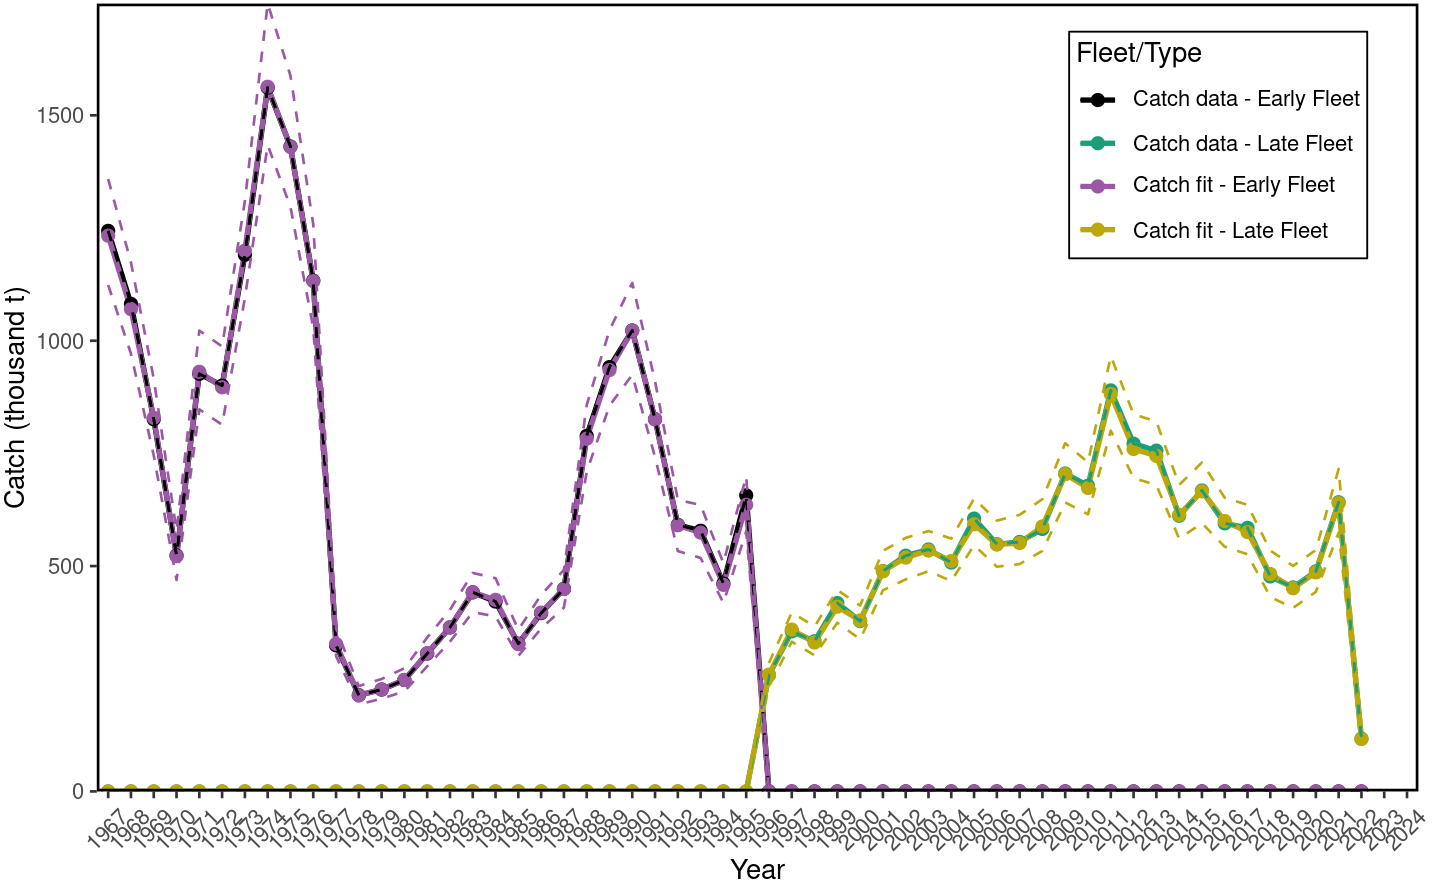
\includegraphics[width=5.5in]{knitr-figs-pdf/fig-catch-fit-1}}{Figure \ref{fig:fig-catch-fit}} 

}

\caption{Predicted catch compared to the observed catch data for the two commercial fleets used in the model. The solid lines are either the observed catches or the median catch by fleet; the dotted lines are the 95\% CI for the posterior of the catch fits.}\label{fig:fig-catch-fit}
\end{figure}



\begin{figure}[H]

{\centering \pdftooltip{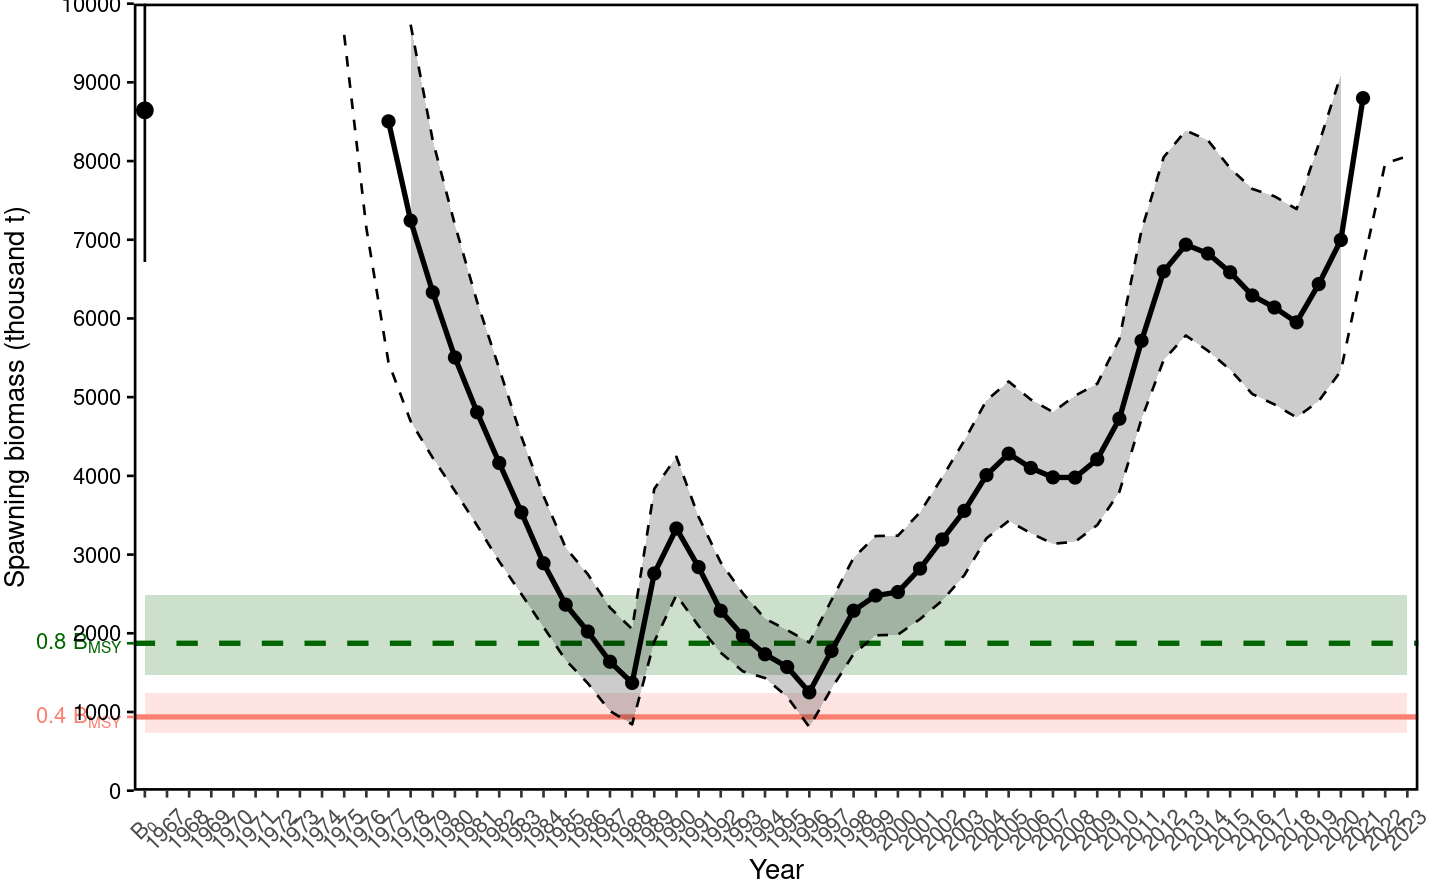
\includegraphics[width=5.5in]{knitr-figs-pdf/fig-base-sb-1}}{Figure \ref{fig:fig-base-sb}} 

}

\caption{Spawning biomass of Petrale sole for the base model with \(B_{MSY}\) reference points. The solid black line with points show the medians of the posteriors, the shaded ribbon encapsulated by dashed lines covers the 95\% CI for the posteriors, the point at \(B_0\) is the median estimate for the unfished biomass, and the vertical line over that point is the 95\% CI for that parameter. The upper part of the CI is not shown for reasons of clarity for the trajectory, the median and CI for \(B_0\) here is 8,644, 6,718--11,220 (width 4,502) thousand t. The \(B_{MSY}\) reference point lines are shown here for reference only, they are not advised for use in decision making for this stock. See section~\ref{scam-ref-points} for more details.}\label{fig:fig-base-sb}
\end{figure}



\begin{figure}[H]

{\centering \pdftooltip{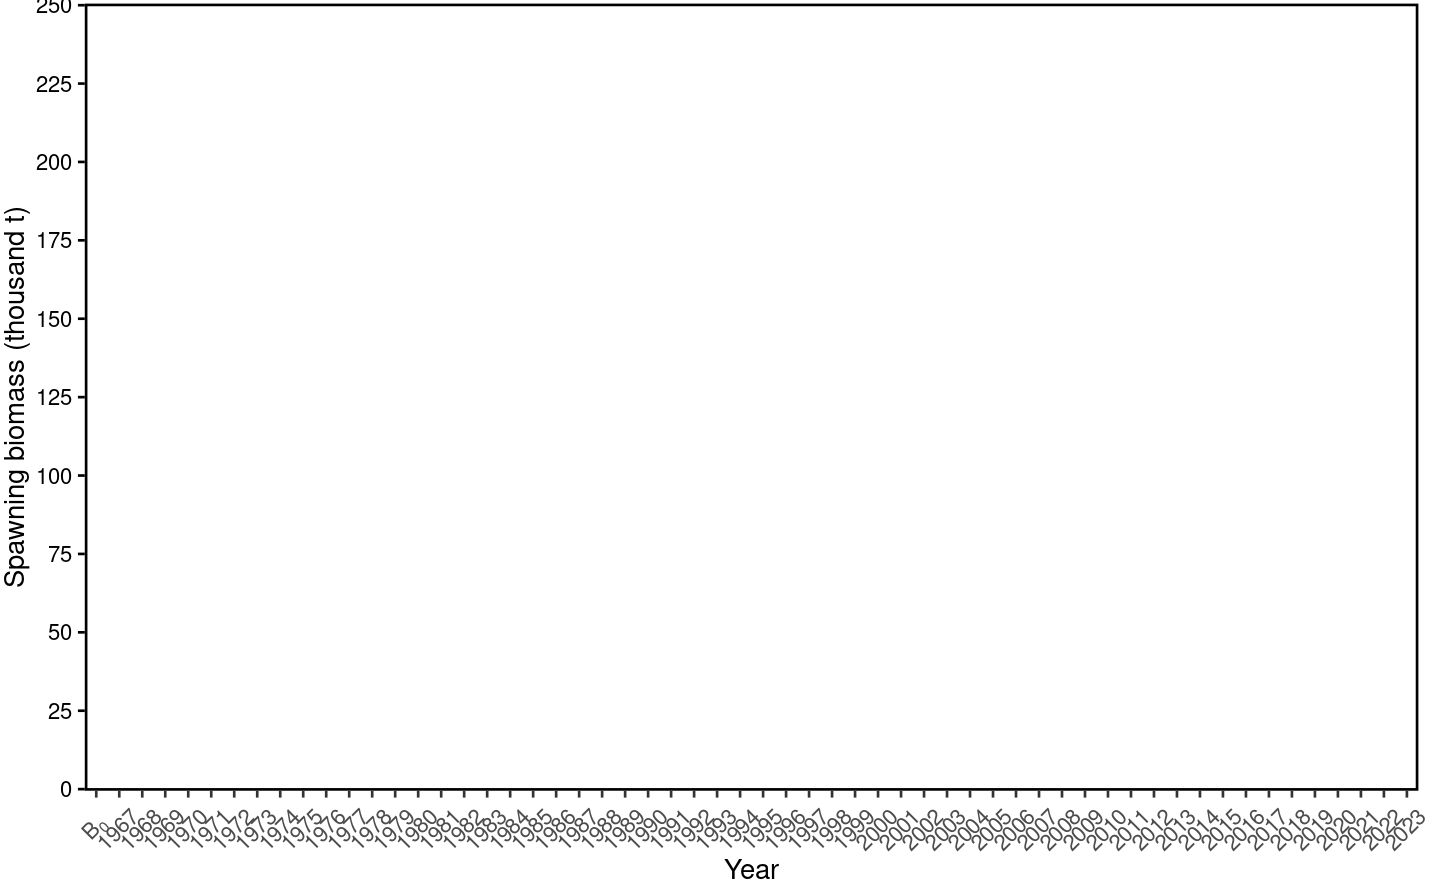
\includegraphics[width=5.5in]{knitr-figs-pdf/fig-base-sb-bo-1}}{Figure \ref{fig:fig-base-sb-bo}} 

}

\caption{Spawning biomass of Petrale sole for the base model with \(B_0\) reference points. See Figure~\ref{fig:fig-base-sb} for more information. The upper part of the CI is not shown for reasons of clarity for the trajectory, the median and CI for \(B_0\) here is 8,644, 6,718--11,220 (width 4,502) thousand t.}\label{fig:fig-base-sb-bo}
\end{figure}



\begin{figure}[H]

{\centering \pdftooltip{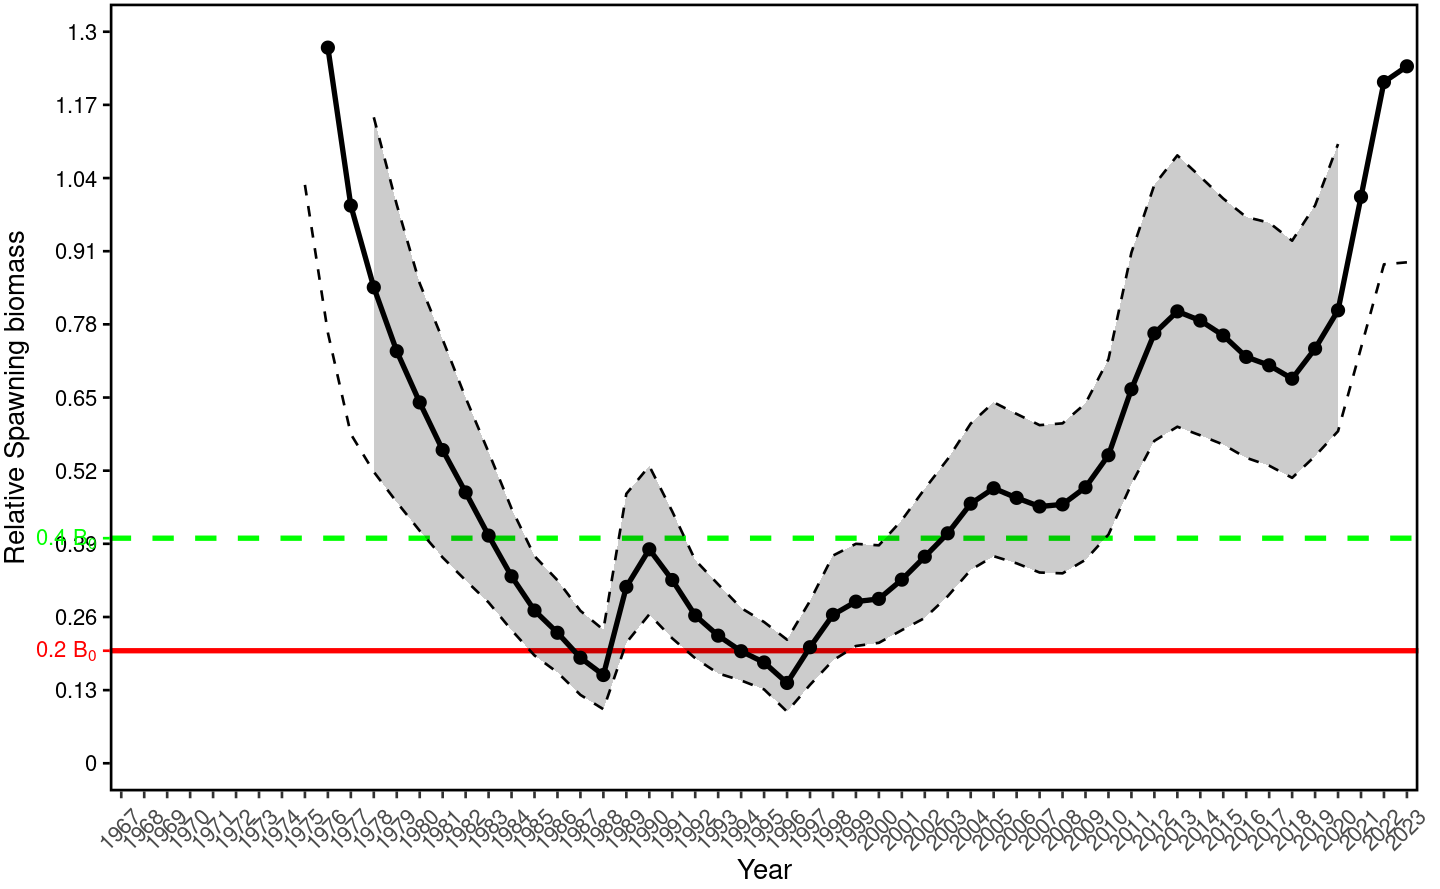
\includegraphics[width=5.5in]{knitr-figs-pdf/fig-base-depletion-1}}{Figure \ref{fig:fig-base-depletion}} 

}

\caption{Relative spawning biomass for the base model. The shaded area represents the 95\% CI. Horizontal lines indicate the 0.2 \(B_0\) (solid, red) and 0.4 \(B_0\) (dashed, green) reference points. Because the ribbon represents relative spawning biomass (depletion) and the reference points are with respect to \(B_0\), all uncertainty about the ratio of the spawning biomass to the reference points is captured in the ribbon and the reference points are shown as point values.}\label{fig:fig-base-depletion}
\end{figure}



\begin{figure}[H]

{\centering \pdftooltip{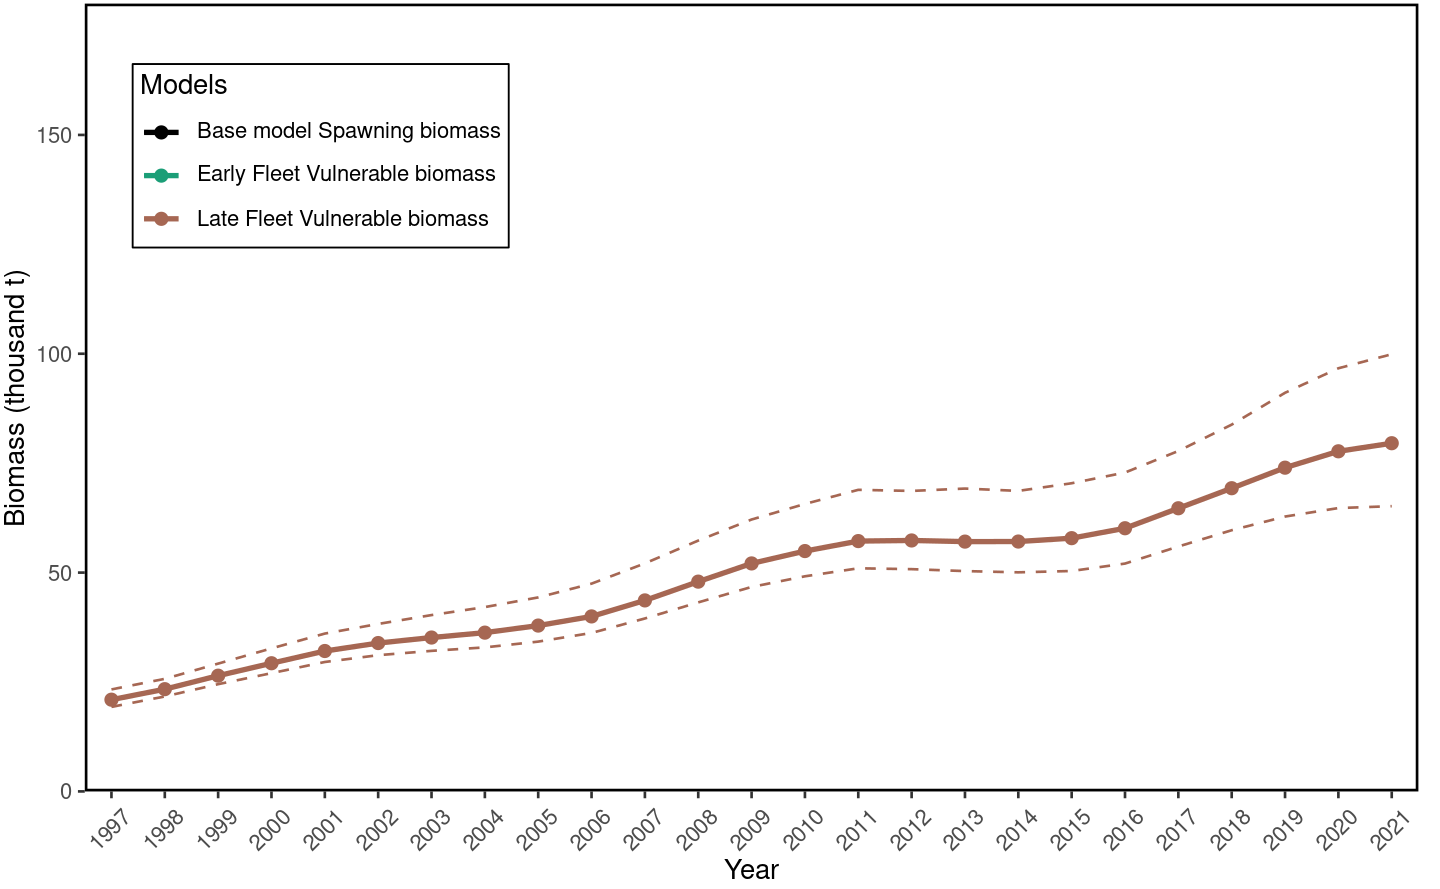
\includegraphics[width=5.5in]{knitr-figs-pdf/fig-base-sb-vuln-compare-1}}{Figure \ref{fig:fig-base-sb-vuln-compare}} 

}

\caption{Spawning biomass of Petrale sole for the base model compared with vulnerable biomass for the trawl fisheries for the base model. The spawning biomass is in black and has its 95\% CI shaded. The two vulnerable biomass trajectories have their 95\% CI contained withing the dotted lines of their respective colours.}\label{fig:fig-base-sb-vuln-compare}
\end{figure}



\begin{figure}[H]

{\centering \pdftooltip{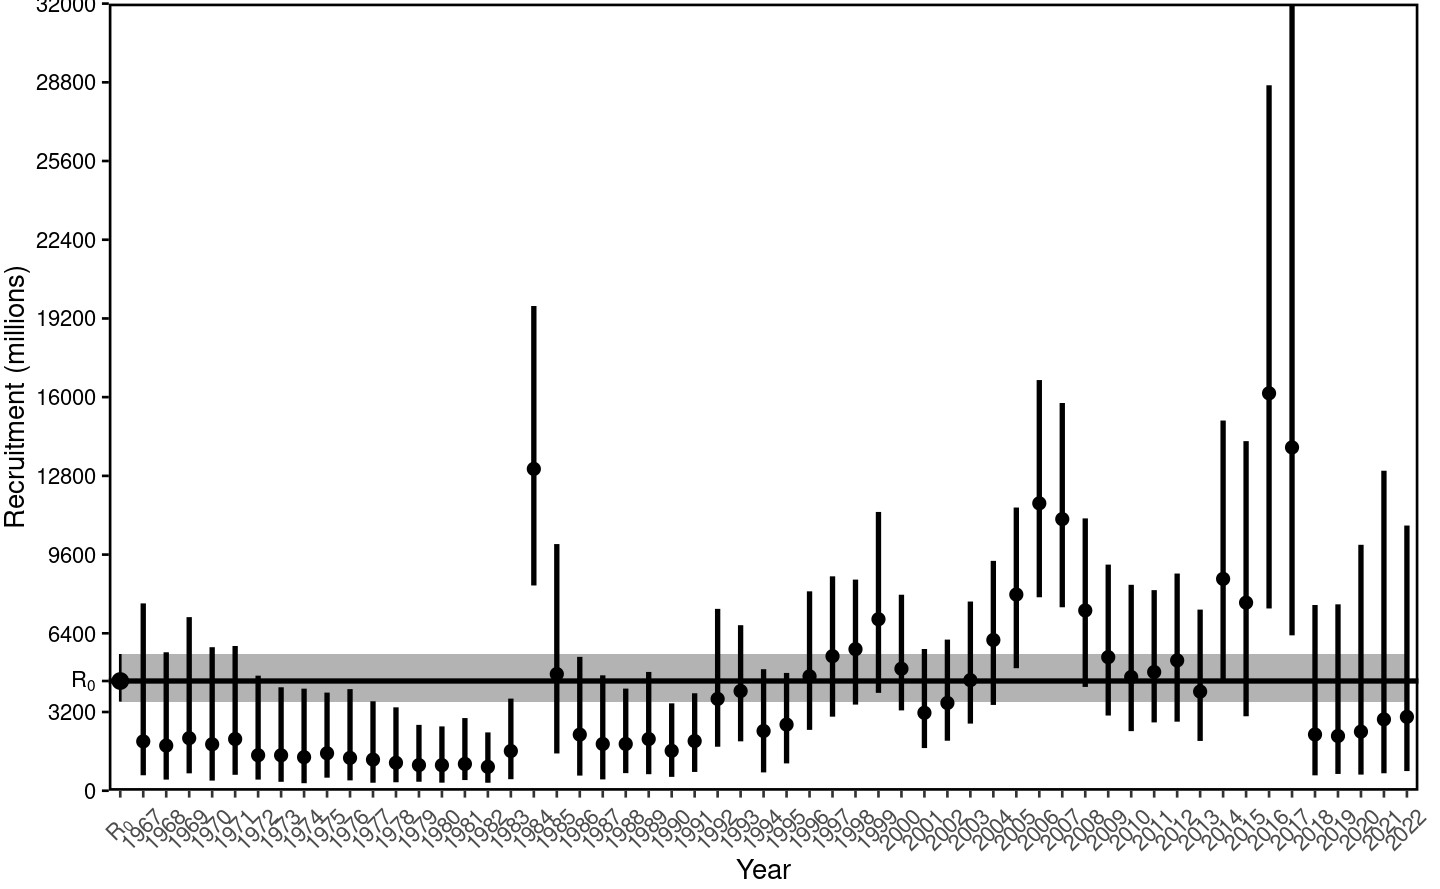
\includegraphics[width=5.5in]{knitr-figs-pdf/fig-base-recr-1}}{Figure \ref{fig:fig-base-recr}} 

}

\caption{Recruitment of Petrale sole for the base model. The black points are the medians of the posteriors, the vertical black lines are the 95\% CIs for the posteriors, the point at \(R_0\) is the median estimate for the initial recruitment parameter \(R_0\), and the vertical line over that point and shaded ribbon across the time series is the 95\% CI for \(R_0\).}\label{fig:fig-base-recr}
\end{figure}



\begin{figure}[H]

{\centering \pdftooltip{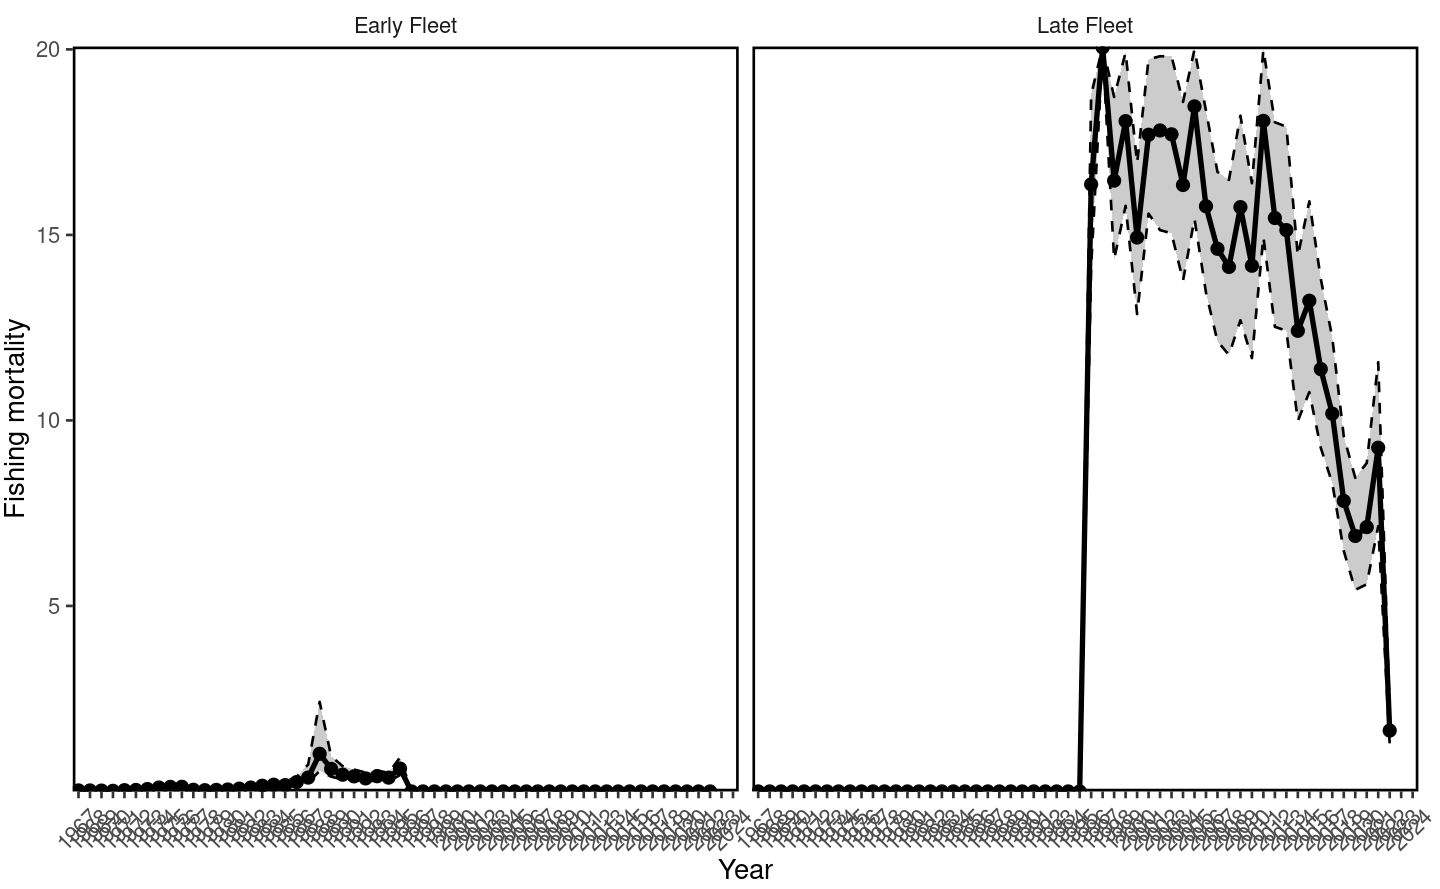
\includegraphics[width=5.5in]{knitr-figs-pdf/fig-base-f-1}}{Figure \ref{fig:fig-base-f}} 

}

\caption{Fishing mortality for the base model for the two trawl fisheries for a single sex. The plots for the second sex are not shown, because they are the same. The shaded area represents the 95\% CI.}\label{fig:fig-base-f}
\end{figure}








\clearpage




\begin{figure}[H]

{\centering \pdftooltip{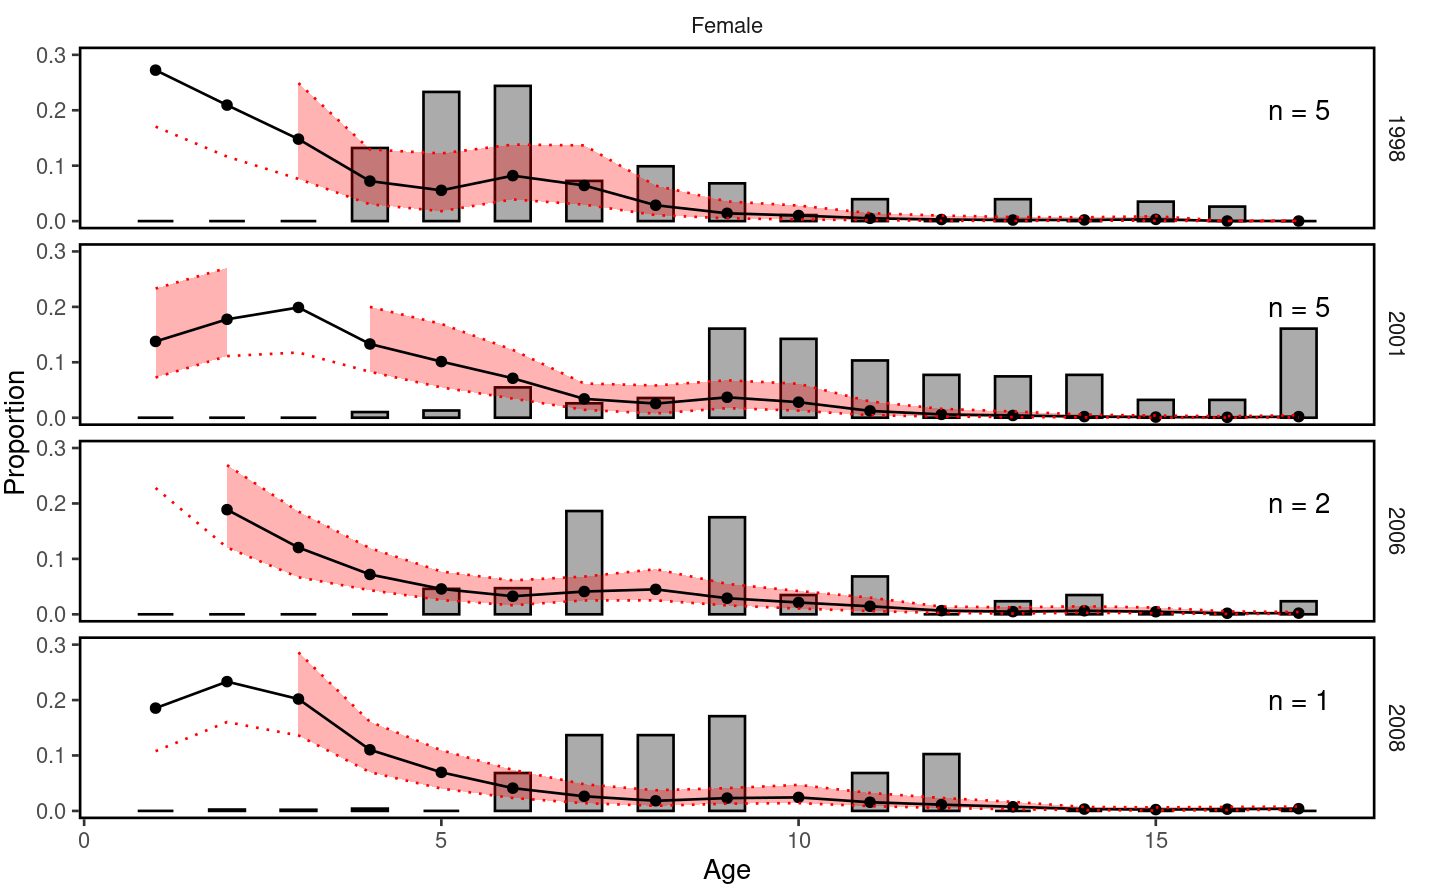
\includegraphics[width=5.5in]{knitr-figs-pdf/fig-base-age-fits-ft-1}}{Figure \ref{fig:fig-base-age-fits-ft}} 

}

\caption{Age composition fits for each sex for the Freezer trawler fleet. The vertical bars are the age composition data points. The sum of the bar values equals 1 for each year/sex combination. The black points are the medians of the posteriors for each age. The red shaded area with dotted edges represents the 95\% CIs. The panel labels are the total number of specimens (sex aggregated) fit for the year.}\label{fig:fig-base-age-fits-ft}
\end{figure}



\begin{figure}[H]

{\centering \pdftooltip{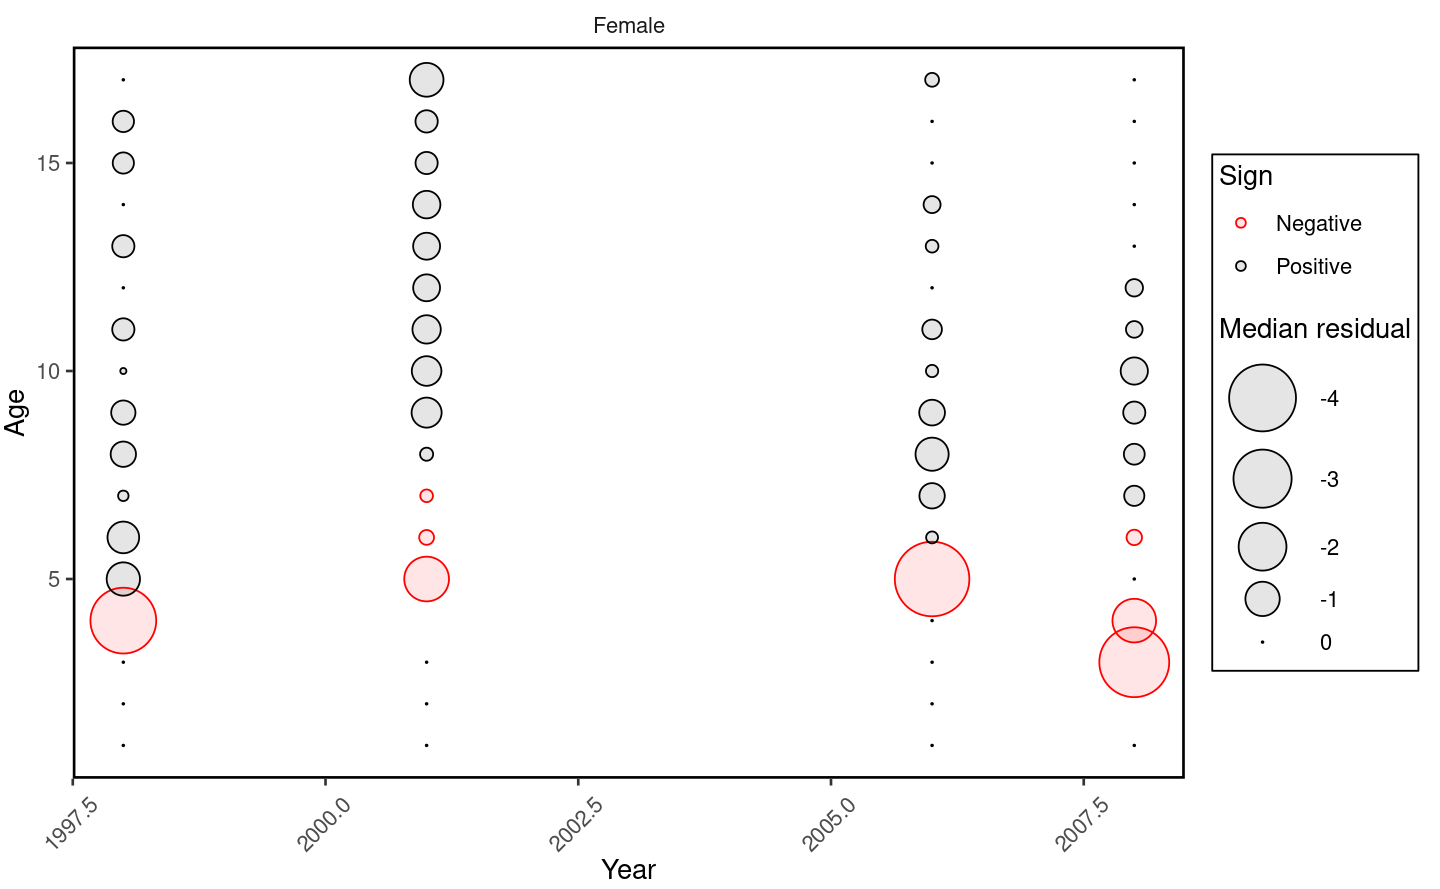
\includegraphics[width=5.5in]{knitr-figs-pdf/fig-base-age-resids-ft-1}}{Figure \ref{fig:fig-base-age-resids-ft}} 

}

\caption{Pearson residuals for the age composition fits for each sex for the Freezer trawler fleet. The bubbles represent the median of the posterior for Pearson residuals. Red bubbles are negative residuals, black are positive, and dots represent zero residuals.}\label{fig:fig-base-age-resids-ft}
\end{figure}
\clearpage




\begin{figure}[H]

{\centering \pdftooltip{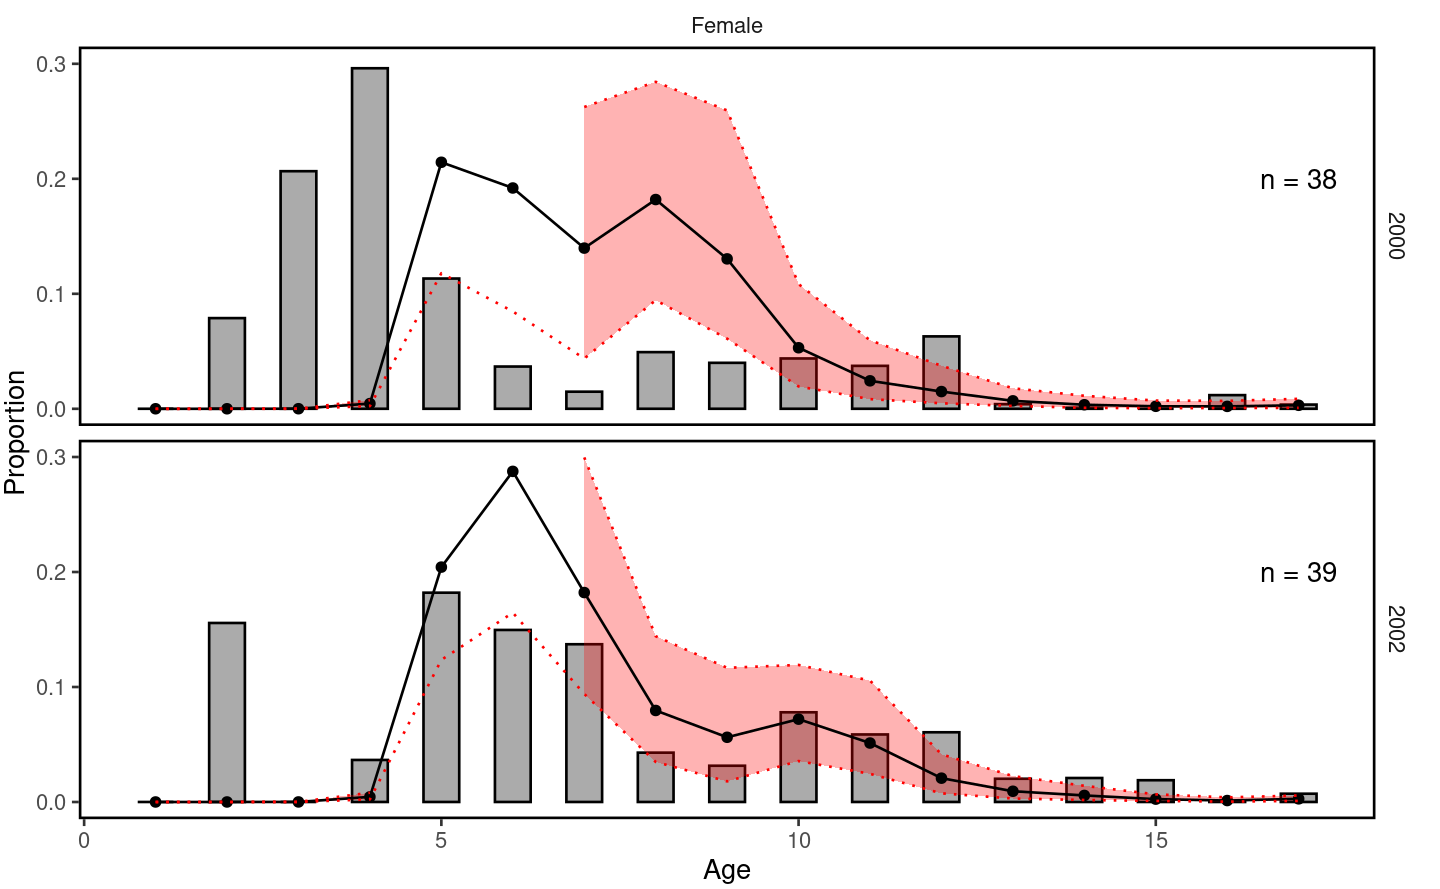
\includegraphics[width=5.5in]{knitr-figs-pdf/fig-base-age-fits-firsthalf-ss-1}}{Figure \ref{fig:fig-base-age-fits-firsthalf-ss}} 

}

\caption{Age composition fits for each sex for the Shoreside fleet from 1996--2007. See Figure~\ref{fig:fig-base-age-fits-ft} for plot details.}\label{fig:fig-base-age-fits-firsthalf-ss}
\end{figure}







\begin{figure}[H]

{\centering \pdftooltip{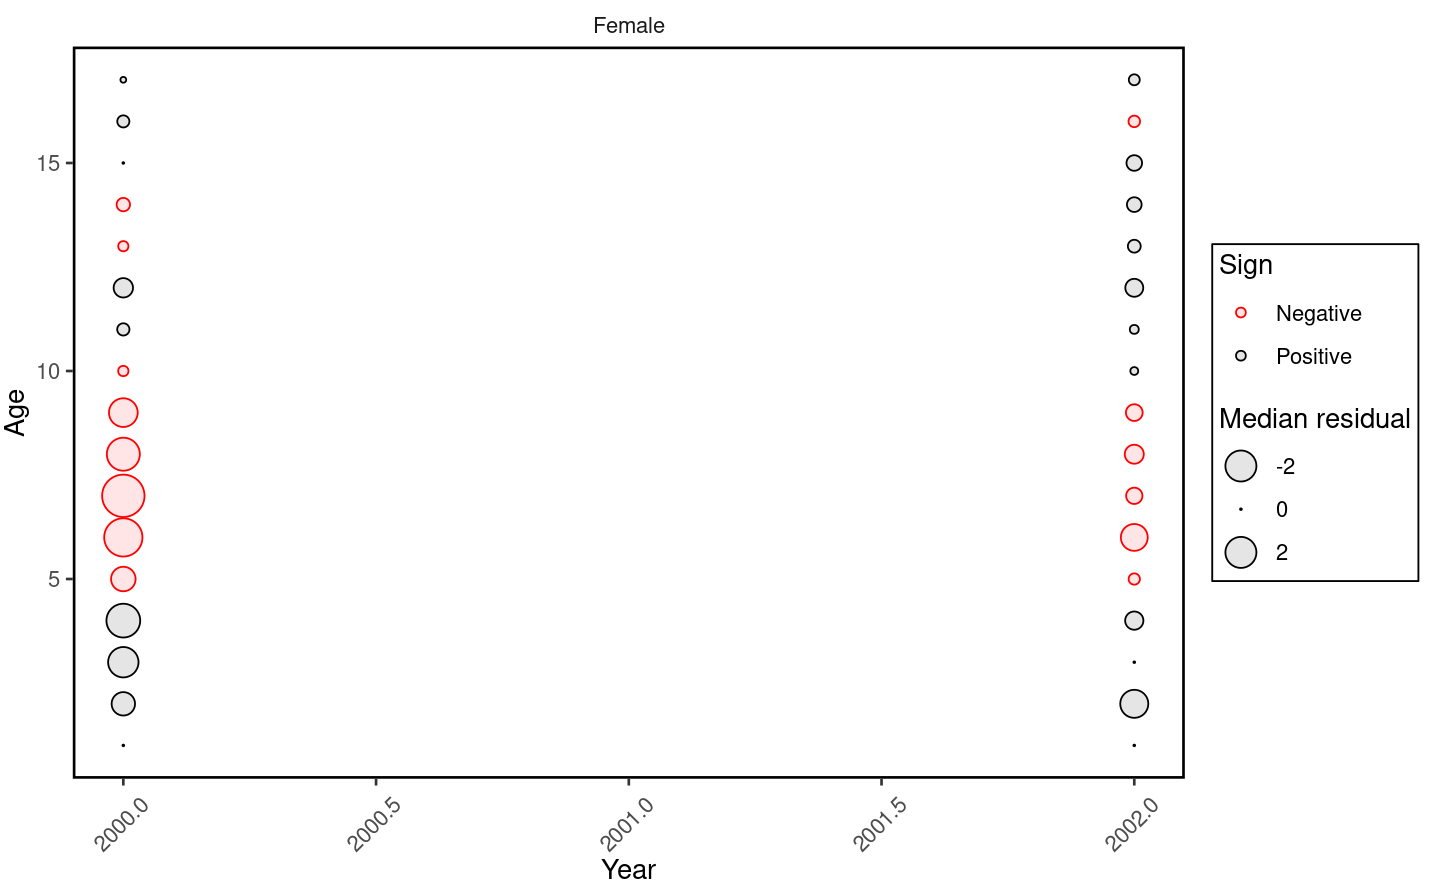
\includegraphics[width=5.5in]{knitr-figs-pdf/fig-base-age-resids-ss-1}}{Figure \ref{fig:fig-base-age-resids-ss}} 

}

\caption{Pearson residuals for the age composition fits for each sex for the Shoreside fleet. The bubbles represent the median of the posterior for Pearson residuals. Red bubbles are negative residuals, black are positive, and dots represent zero residuals.}\label{fig:fig-base-age-resids-ss}
\end{figure}
\clearpage




\begin{figure}[H]

{\centering \pdftooltip{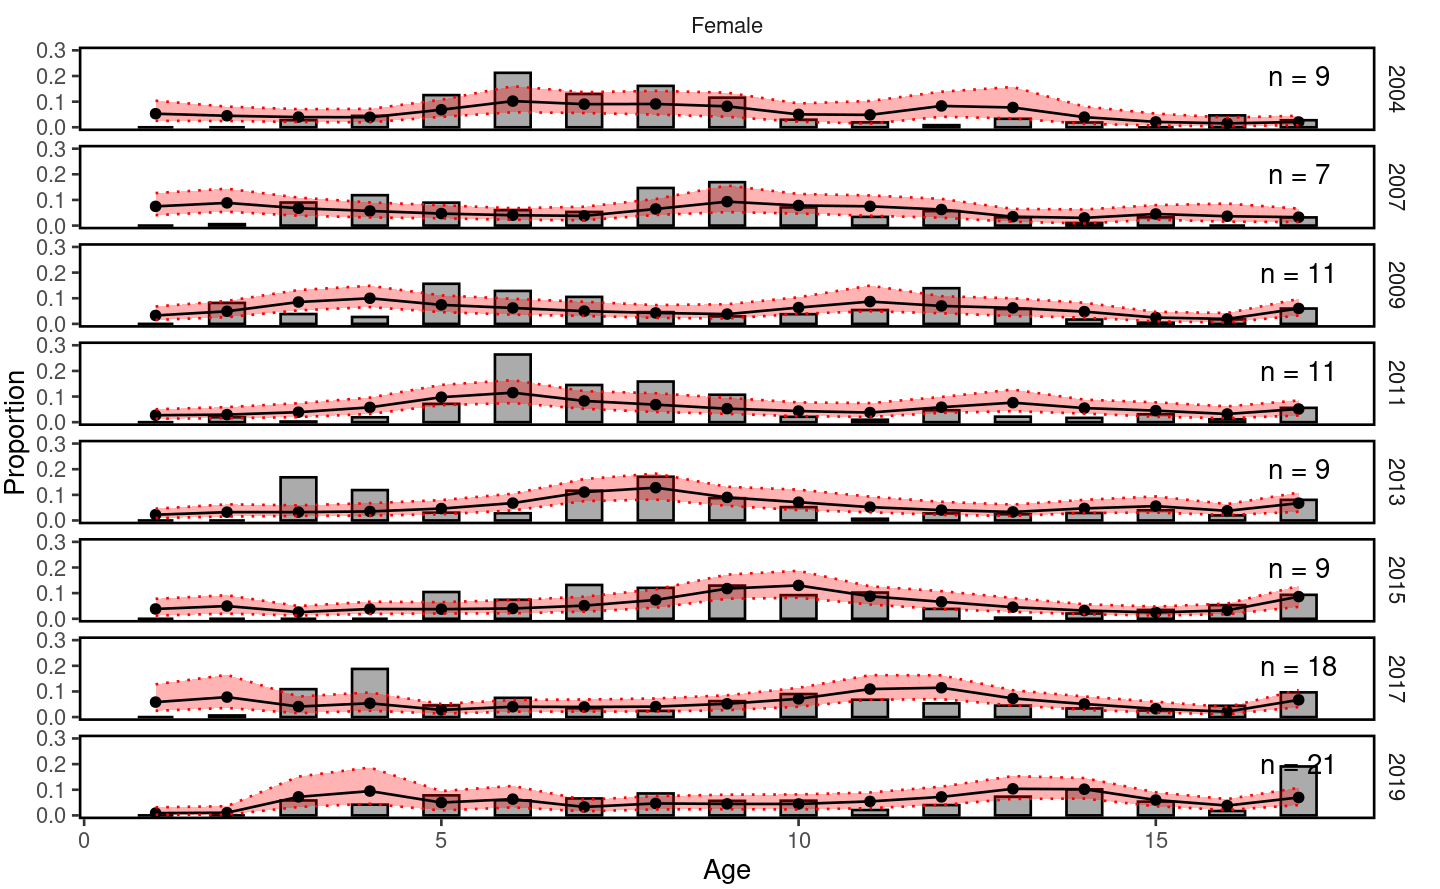
\includegraphics[width=5.5in]{knitr-figs-pdf/fig-base-age-fits-qcs-1}}{Figure \ref{fig:fig-base-age-fits-qcs}} 

}

\caption{Age composition fits for each sex for the Queen Charlotte Sound Synoptic Survey. See Figure~\ref{fig:fig-base-age-fits-ft} for plot details.}\label{fig:fig-base-age-fits-qcs}
\end{figure}



\begin{figure}[H]

{\centering \pdftooltip{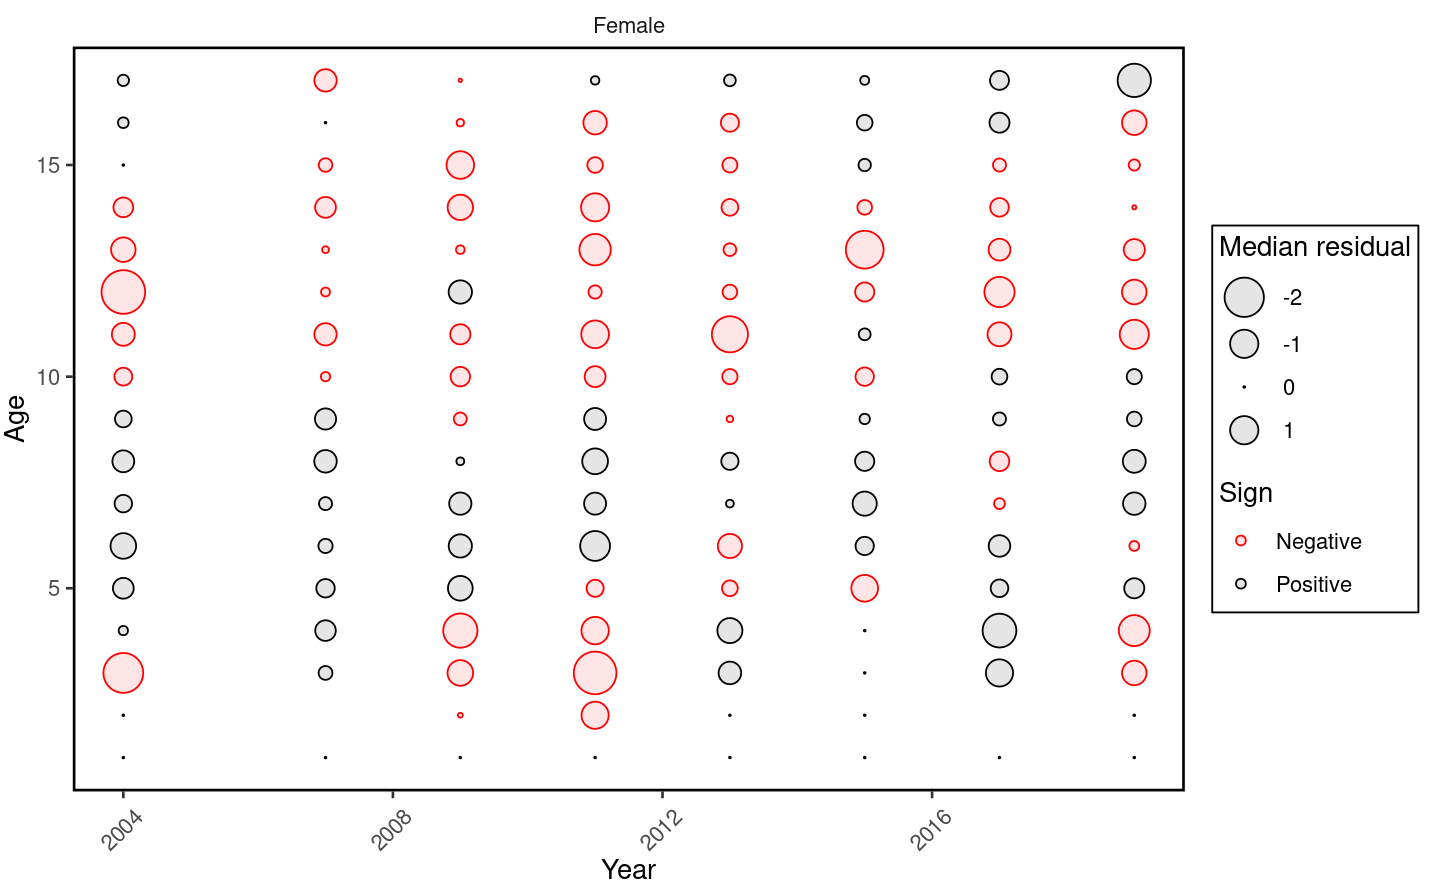
\includegraphics[width=5.5in]{knitr-figs-pdf/fig-base-age-resids-qcs-1}}{Figure \ref{fig:fig-base-age-resids-qcs}} 

}

\caption{Pearson residuals for the age composition fits for each sex for the Queen Charlotte Sound Synoptic Survey. The bubbles represent the median of the posterior for Pearson residuals. Red bubbles are negative residuals, black are positive, and dots represent zero residuals.}\label{fig:fig-base-age-resids-qcs}
\end{figure}
\clearpage




\begin{figure}[H]

{\centering \pdftooltip{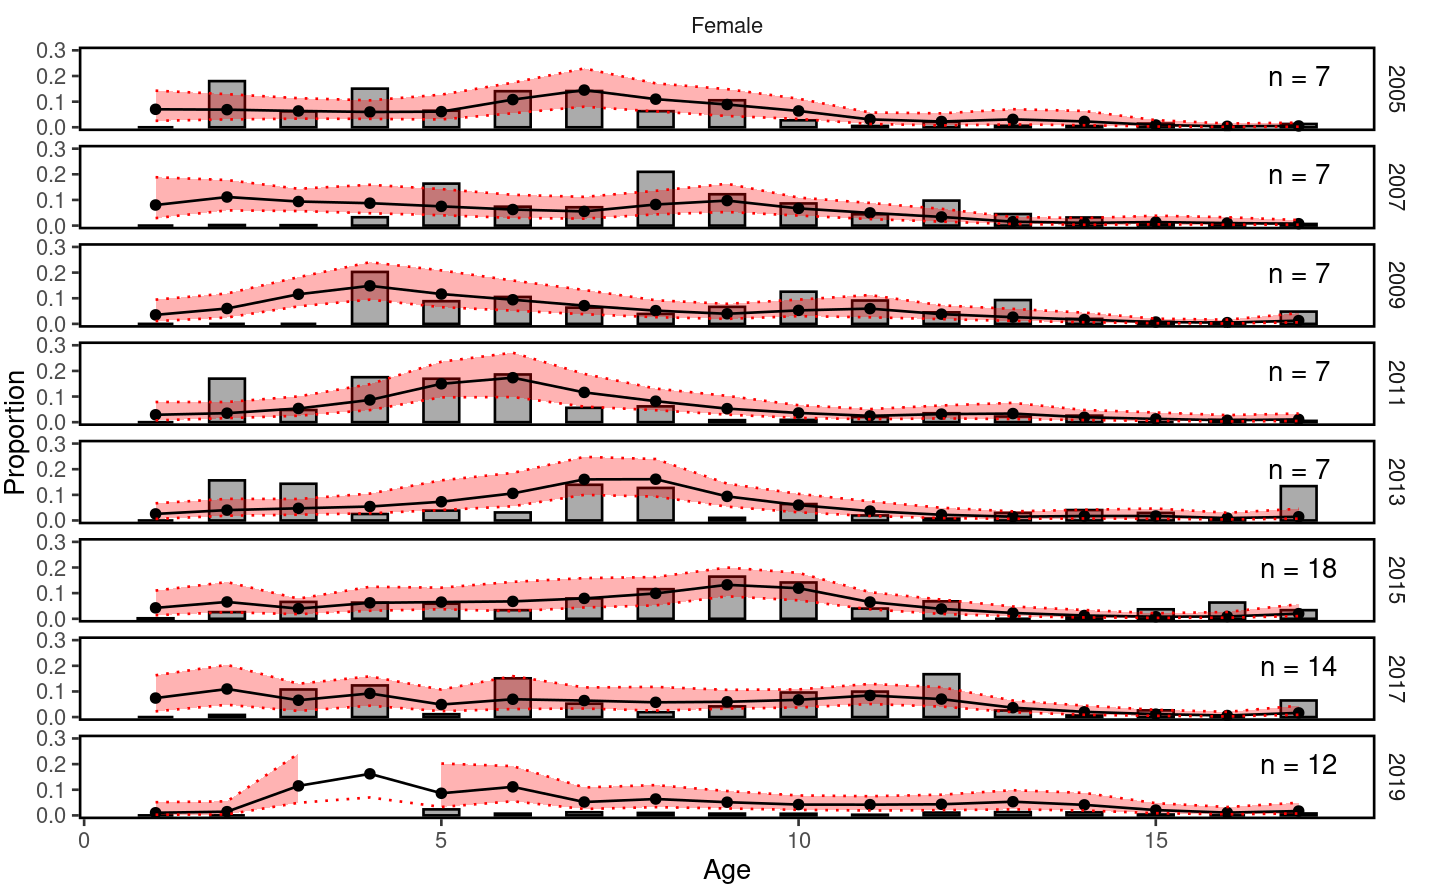
\includegraphics[width=5.5in]{knitr-figs-pdf/fig-base-age-fits-hss-1}}{Figure \ref{fig:fig-base-age-fits-hss}} 

}

\caption{Age composition fits for each sex for the Hecate Strait Synoptic Survey. See Figure~\ref{fig:fig-base-age-fits-ft} for plot details.}\label{fig:fig-base-age-fits-hss}
\end{figure}



\begin{figure}[H]

{\centering \pdftooltip{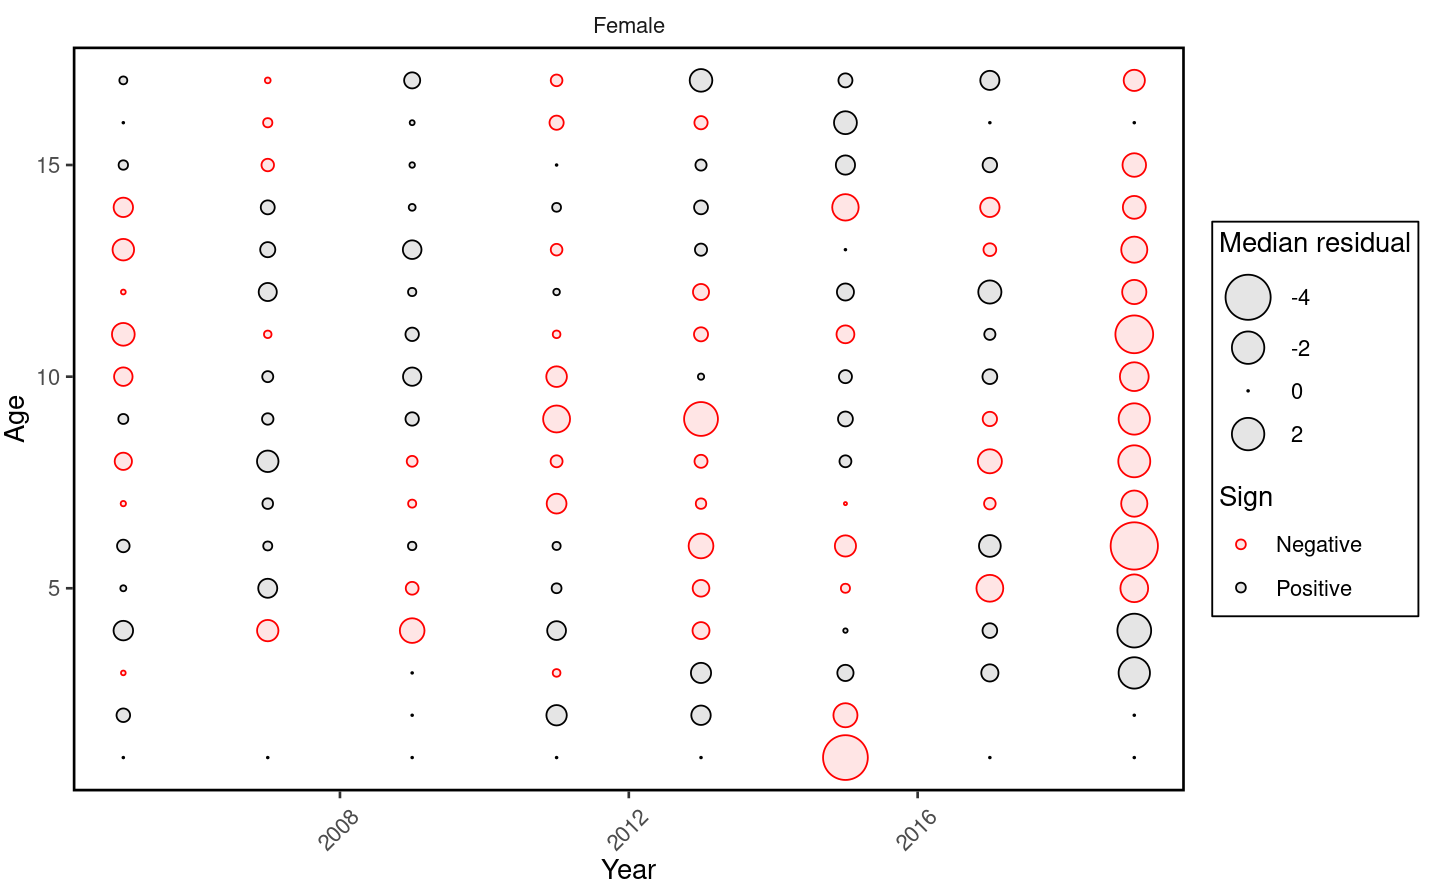
\includegraphics[width=5.5in]{knitr-figs-pdf/fig-base-age-resids-hss-1}}{Figure \ref{fig:fig-base-age-resids-hss}} 

}

\caption{Pearson residuals for the age composition fits for each sex for the Hecate Strait Synoptic Survey. The bubbles represent the median of the posterior for Pearson residuals. Red bubbles are negative residuals, black are positive, and dots represent zero residuals.}\label{fig:fig-base-age-resids-hss}
\end{figure}
\clearpage




\begin{figure}[H]

{\centering \pdftooltip{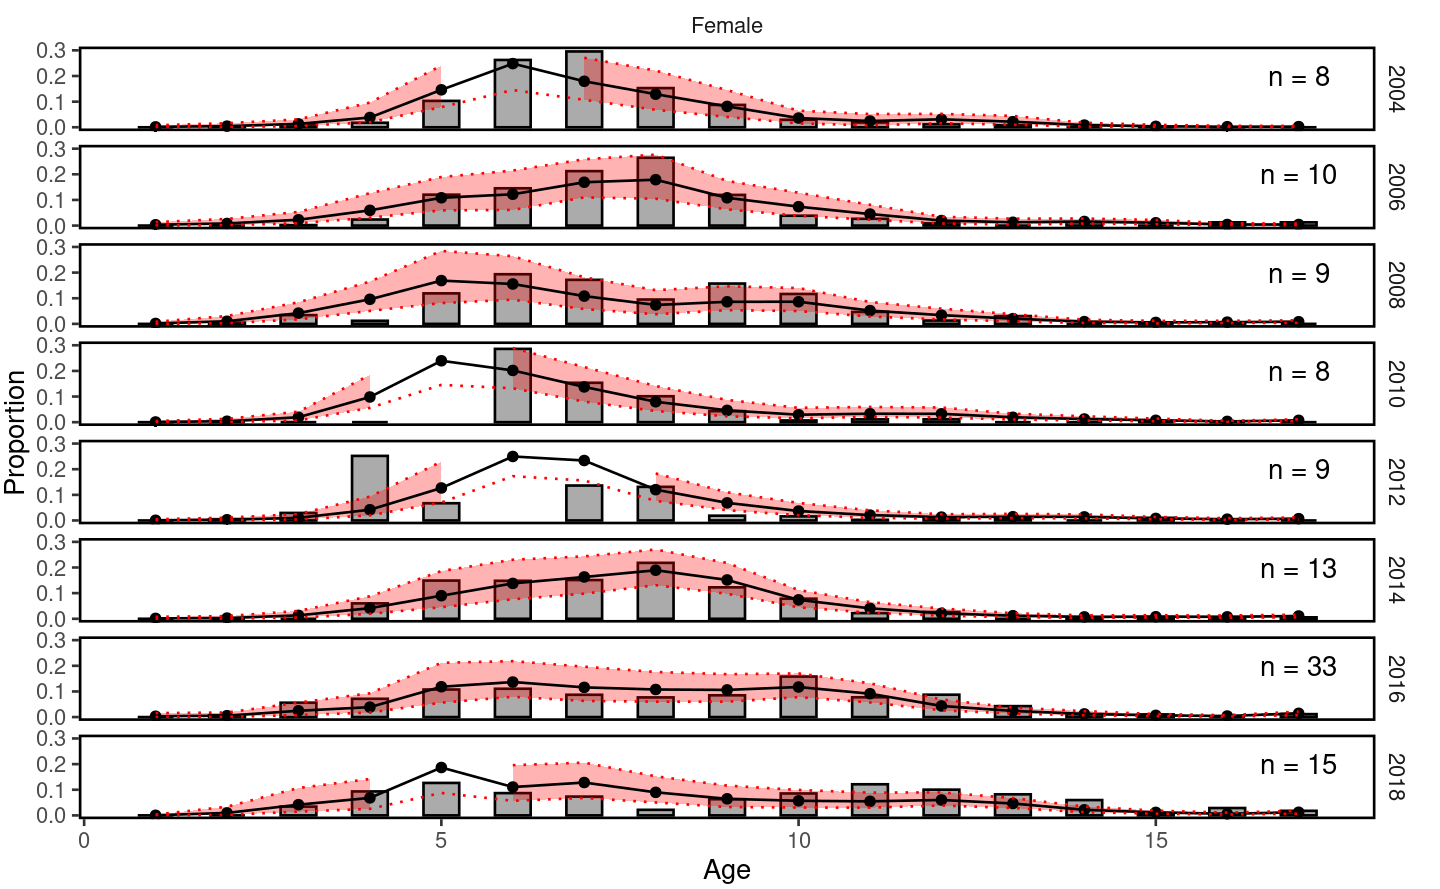
\includegraphics[width=5.5in]{knitr-figs-pdf/fig-base-age-fits-wcvis-1}}{Figure \ref{fig:fig-base-age-fits-wcvis}} 

}

\caption{Age composition fits for each sex for the West Coast Vancouver Island Synoptic Survey. See Figure~\ref{fig:fig-base-age-fits-ft} for plot details.}\label{fig:fig-base-age-fits-wcvis}
\end{figure}



\begin{figure}[H]

{\centering \pdftooltip{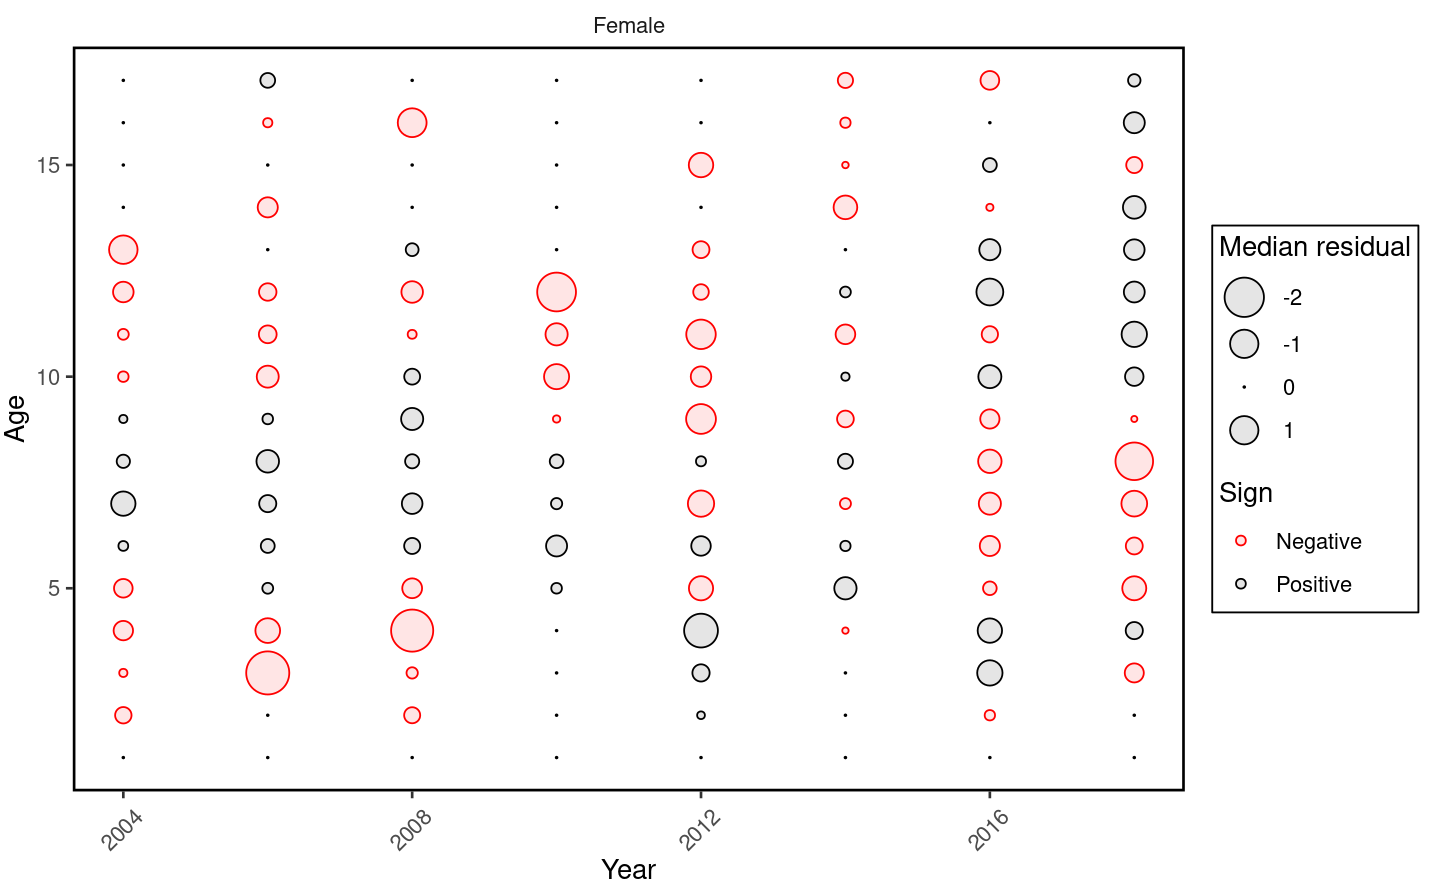
\includegraphics[width=5.5in]{knitr-figs-pdf/fig-base-age-resids-wcvis-1}}{Figure \ref{fig:fig-base-age-resids-wcvis}} 

}

\caption{Pearson residuals for the age composition fits for each sex for the West Coast Vancouver Island Synoptic Survey. The bubbles represent the median of the posterior for Pearson residuals. Red bubbles are negative residuals, black are positive, and dots represent zero residuals.}\label{fig:fig-base-age-resids-wcvis}
\end{figure}
\clearpage

\clearpage




\begin{figure}[H]

{\centering \pdftooltip{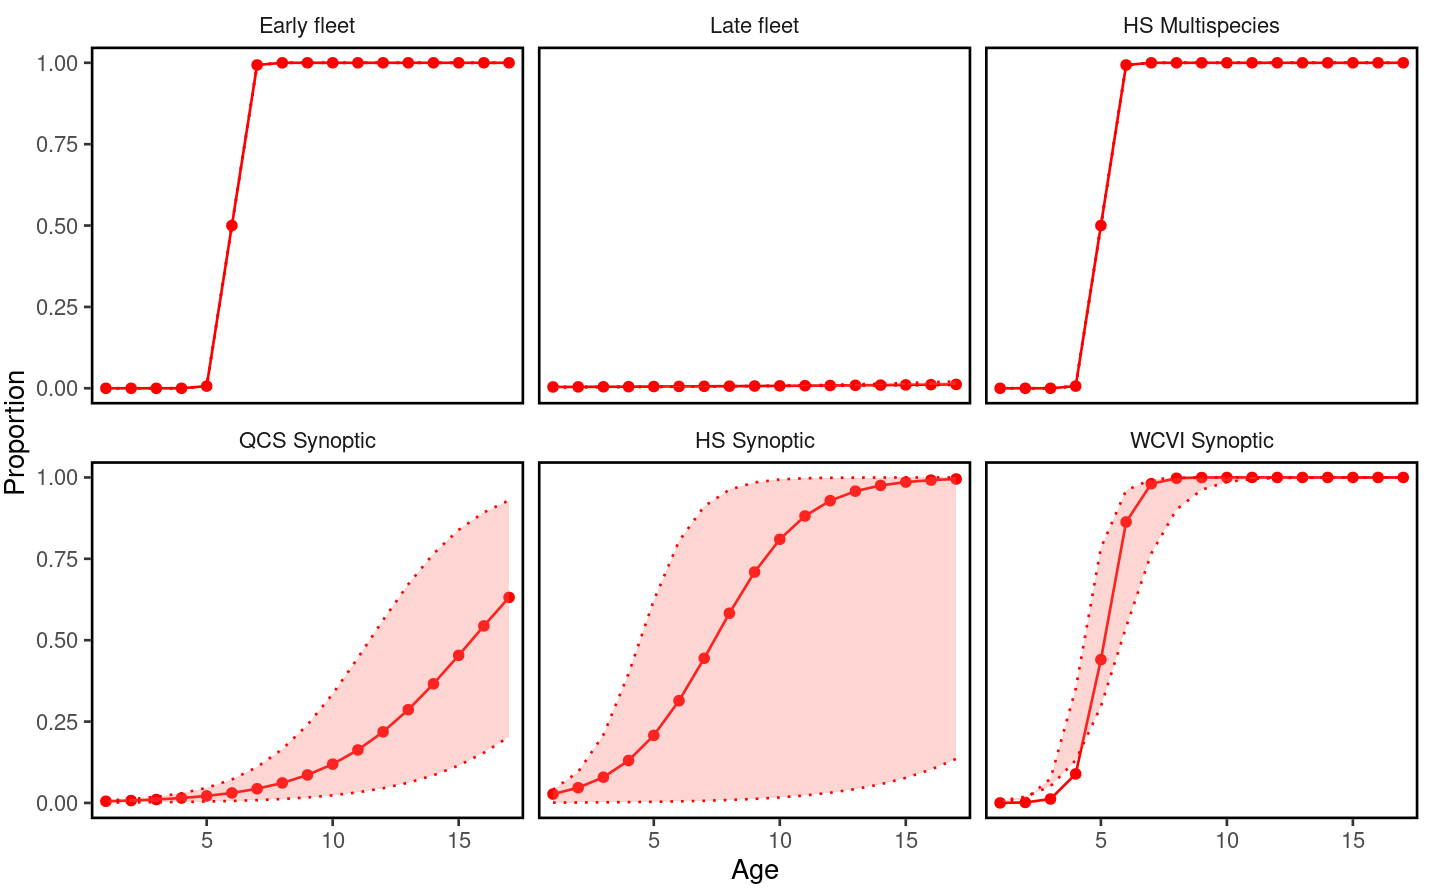
\includegraphics[width=5.5in]{knitr-figs-pdf/fig-base-mcmc-selex-1}}{Figure \ref{fig:fig-base-mcmc-selex}} 

}

\caption{Estimated and fixed selectivities by sex for the base model. The dots are estimated selectivity-at-age, the shaded areas around are the 95\% CI for those estimates. Single lines with no CI are fixed selectivities. Dashed lines represent maturity, with the colours representing the sexes and are the same as for selectivity curves.}\label{fig:fig-base-mcmc-selex}
\end{figure}



\begin{figure}[H]

{\centering \pdftooltip{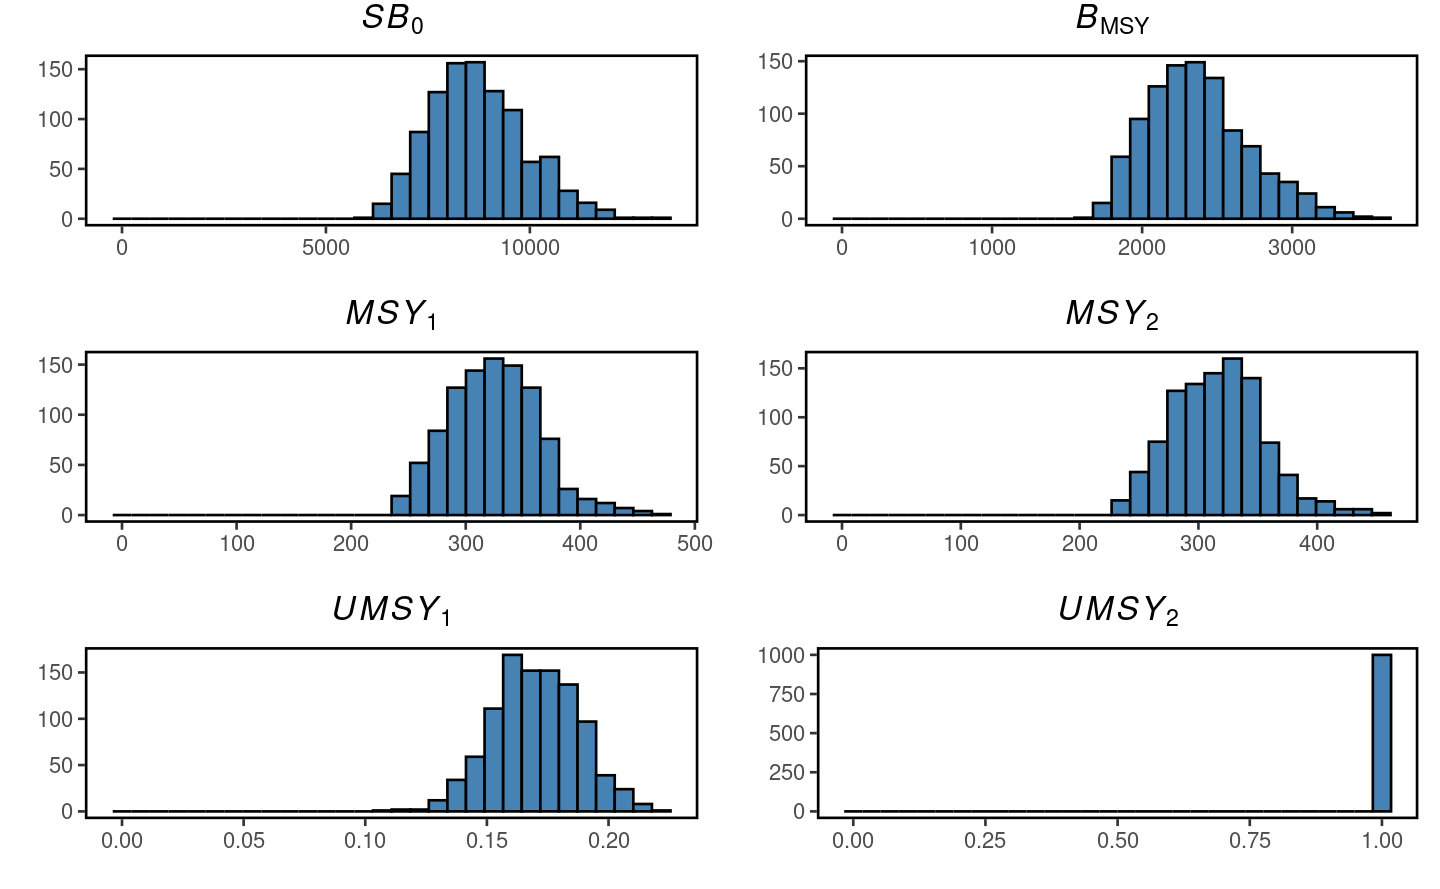
\includegraphics[width=5.5in]{knitr-figs-pdf/fig-base-ref-points-1}}{Figure \ref{fig:fig-base-ref-points}} 

}

\caption{Posterior distributions for reference points and other values of interest for the base model. Subscripts are 1 = Freezer trawlers and 2 = Shoreside.}\label{fig:fig-base-ref-points}
\end{figure}
\clearpage

\hypertarget{mcmc-diagnostic-figures-for-the-base-model}{%
\subsection{MCMC DIAGNOSTIC FIGURES FOR THE BASE MODEL}\label{mcmc-diagnostic-figures-for-the-base-model}}








\begin{figure}[H]

{\centering \pdftooltip{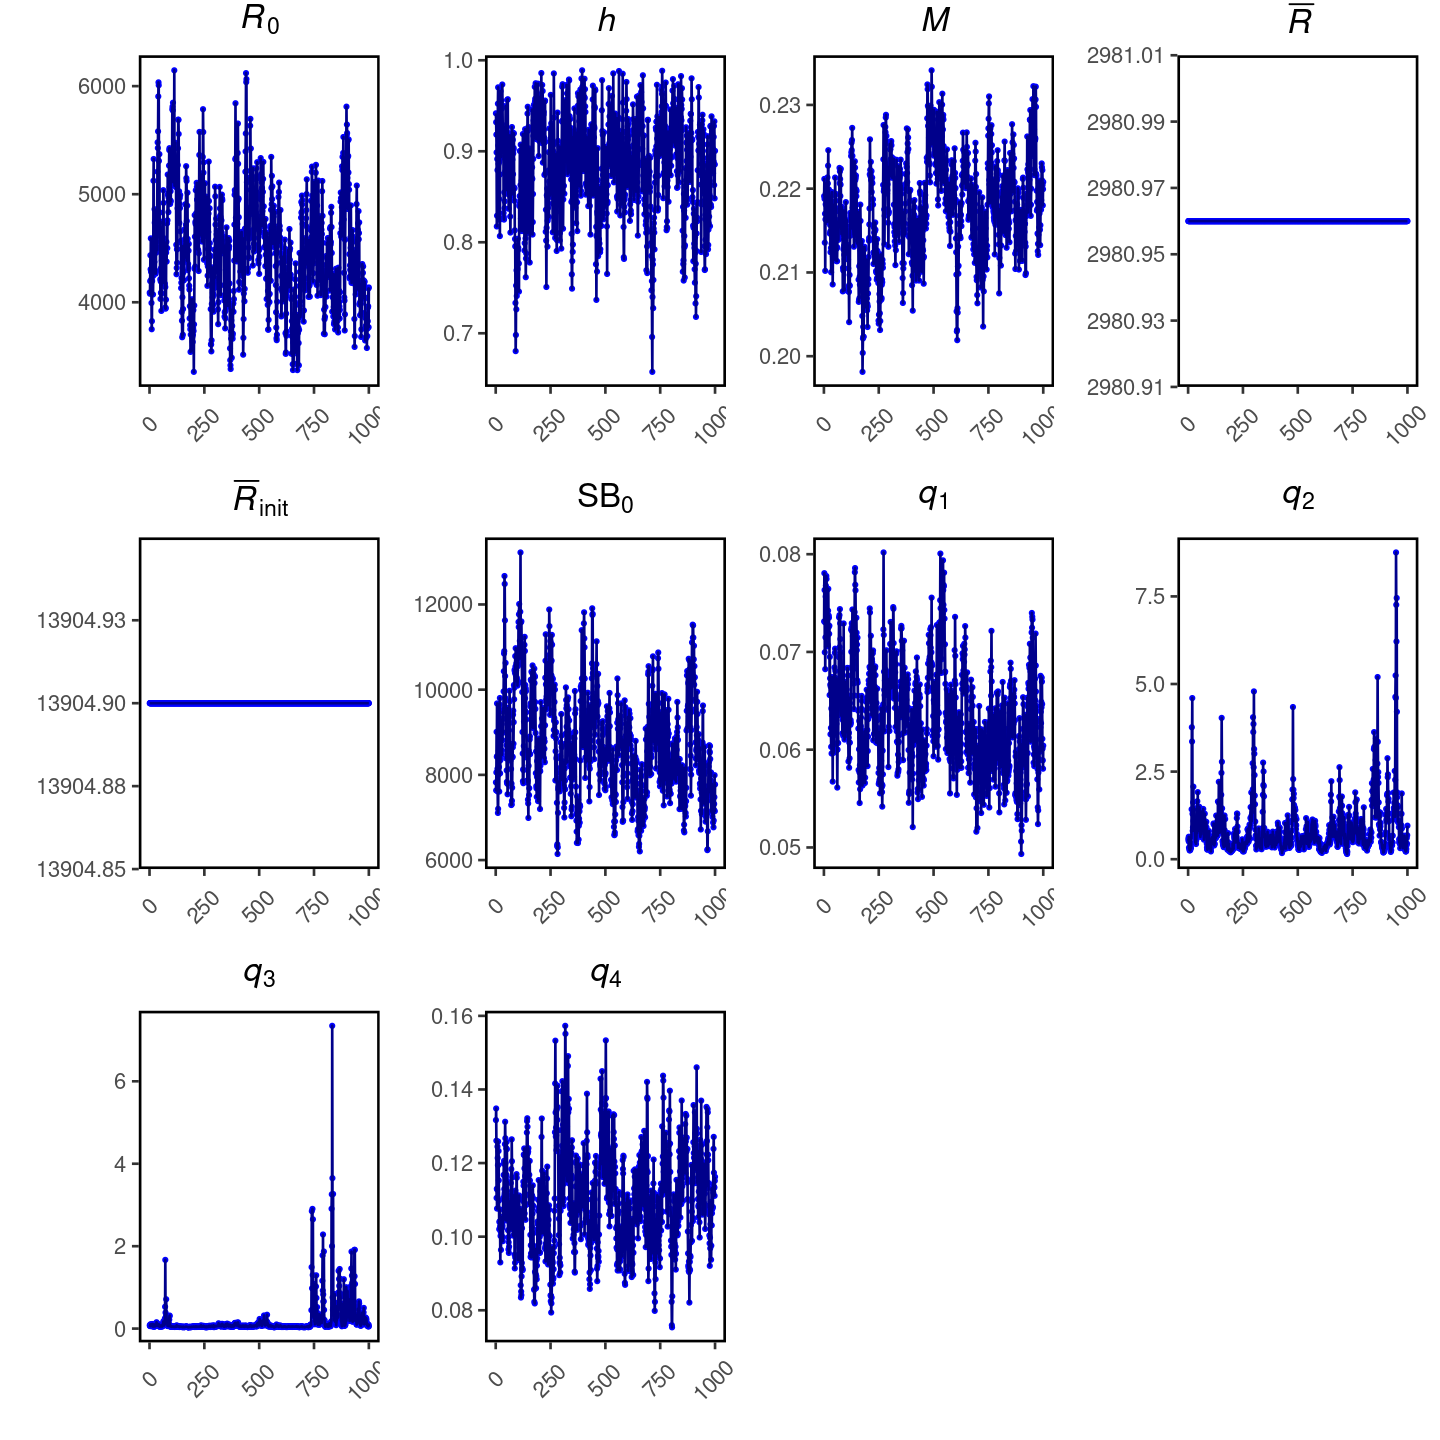
\includegraphics[width=5.5in]{knitr-figs-pdf/fig-base-trace-1}}{Figure \ref{fig:fig-base-trace}} 

}

\caption{Trace plots for MCMC output of estimated lead parameters in the base model. The MCMC run has chain length 10,000,000 with a sample taken every 5,000\textsuperscript{th} iteration. Of the 2,000 samples taken, the first 1,000 were removed as a burn-in period. See Figure~\ref{fig:fig-base-priors-posts} for \(q\) subscript descriptions.}\label{fig:fig-base-trace}
\end{figure}



\begin{figure}[H]

{\centering \pdftooltip{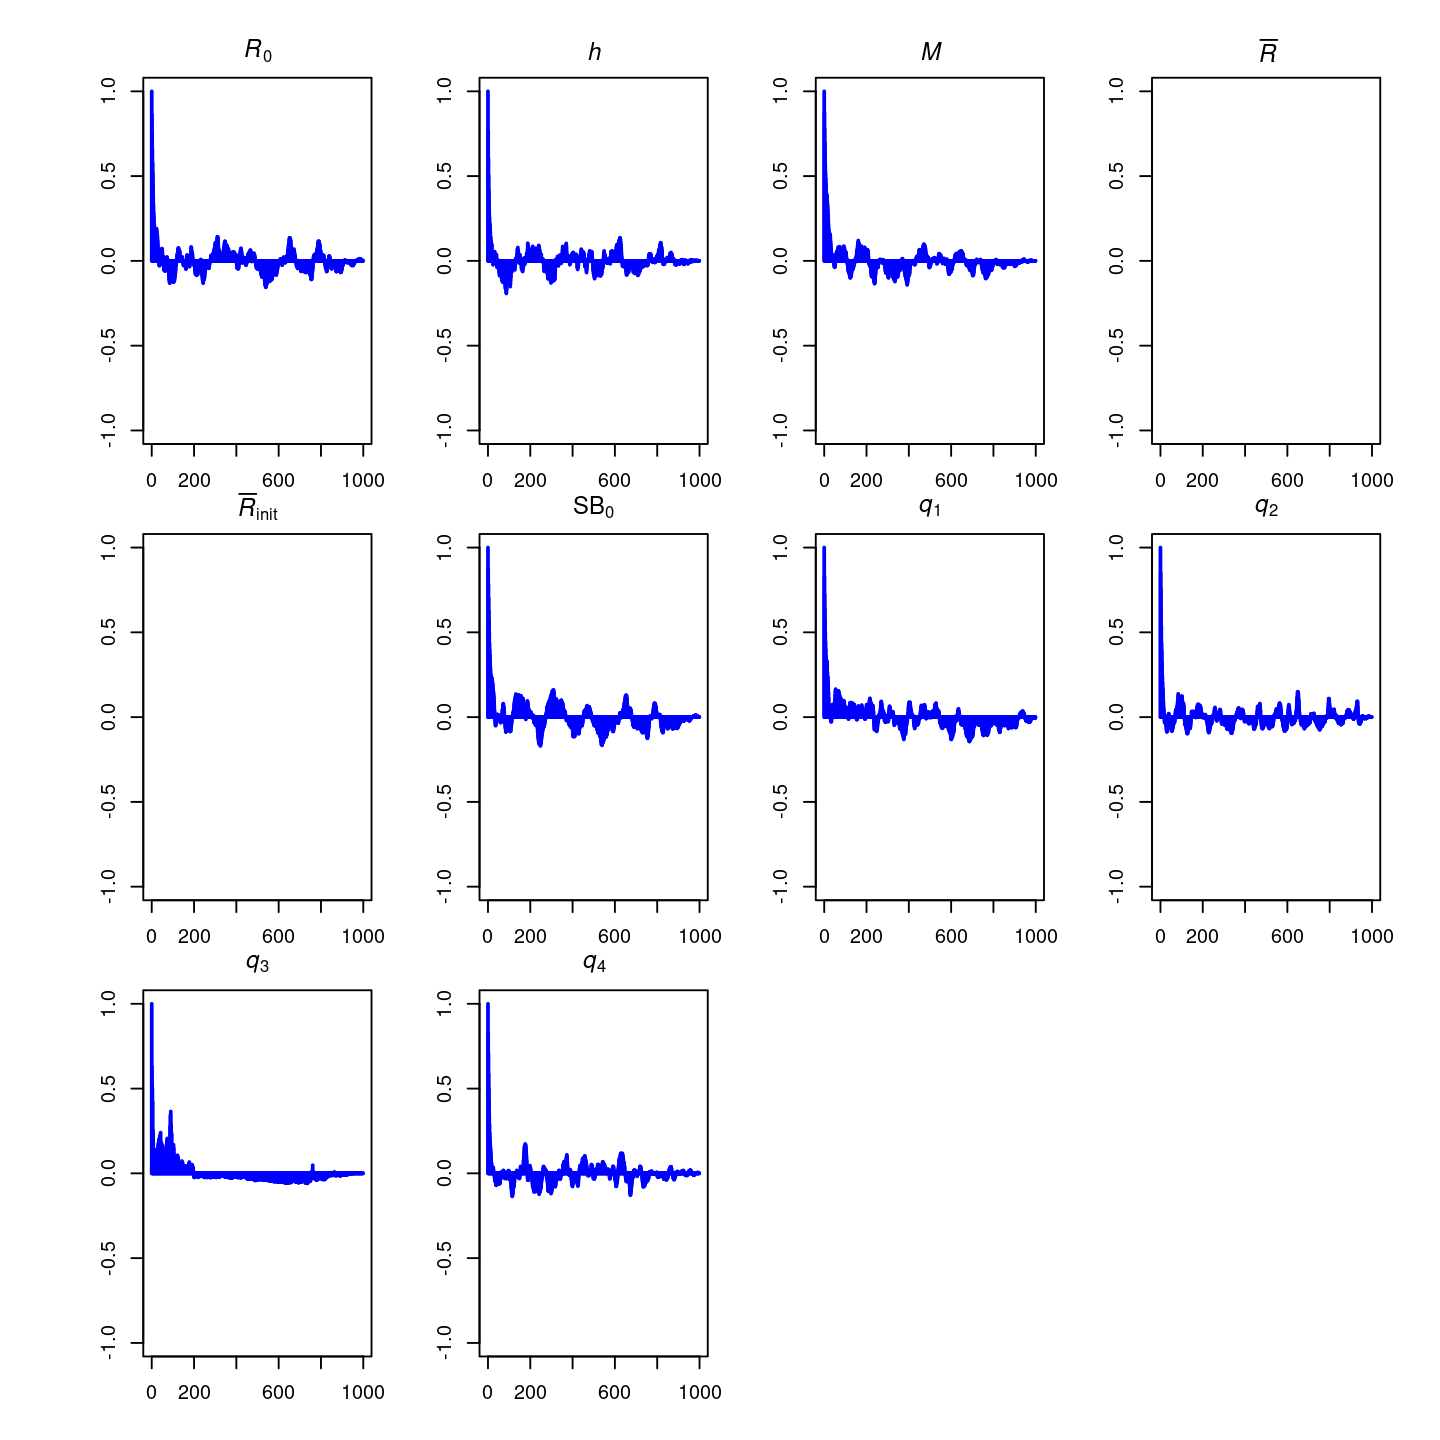
\includegraphics[width=5.5in]{knitr-figs-pdf/fig-base-autocor-1}}{Figure \ref{fig:fig-base-autocor}} 

}

\caption{Autocorrelation plots for MCMC output of estimated lead parameters in the base model. The x-axis values are the lag between posteriors. See Figure~\ref{fig:fig-base-priors-posts} for \(q\) subscript descriptions.}\label{fig:fig-base-autocor}
\end{figure}



\begin{figure}[H]

{\centering \pdftooltip{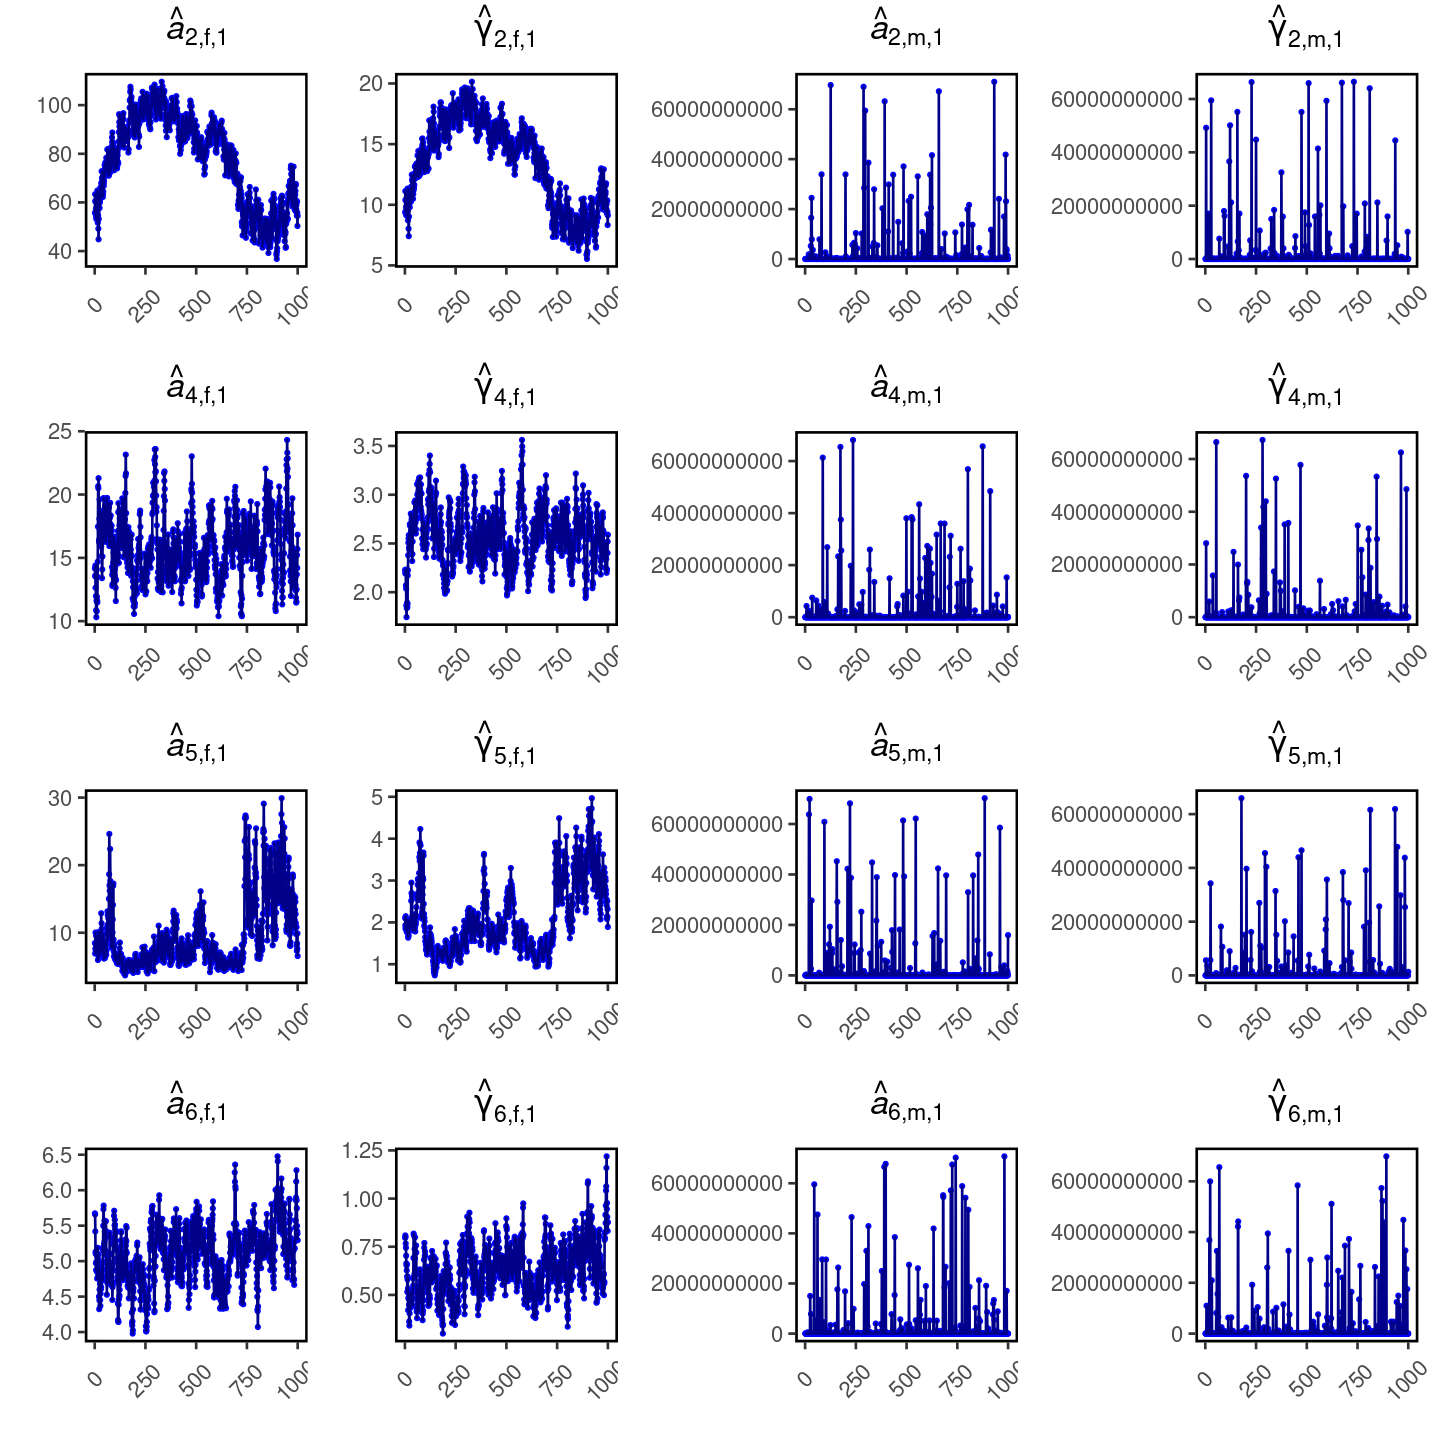
\includegraphics[width=5.5in]{knitr-figs-pdf/fig-base-trace-selex-1}}{Figure \ref{fig:fig-base-trace-selex}} 

}

\caption{Trace plots for MCMC output of estimated selectivity parameters in the base model. \(\hat{a}\) are the estimates of selectivity-at-age-50\%, \(\hat{\gamma}\) are the estimated standard deviations on selectivity-at-age-50\%. The first numerical subscript is the gear number which are: 1 = Early fleet, 2 = Late fleet, 3 = HS Multispecies, 4 = QCS Synoptic, 5 = HS Synoptic, 6 = WCVI Synoptic. The letter subscripts `f' and `m' correspond to female and male, and the second numerical subscripts represent the year block for selectivity. For the base model, there is only the subscript `1' for all parameters shown, because time-varying selectivity was not implemented.}\label{fig:fig-base-trace-selex}
\end{figure}



\begin{figure}[H]

{\centering \pdftooltip{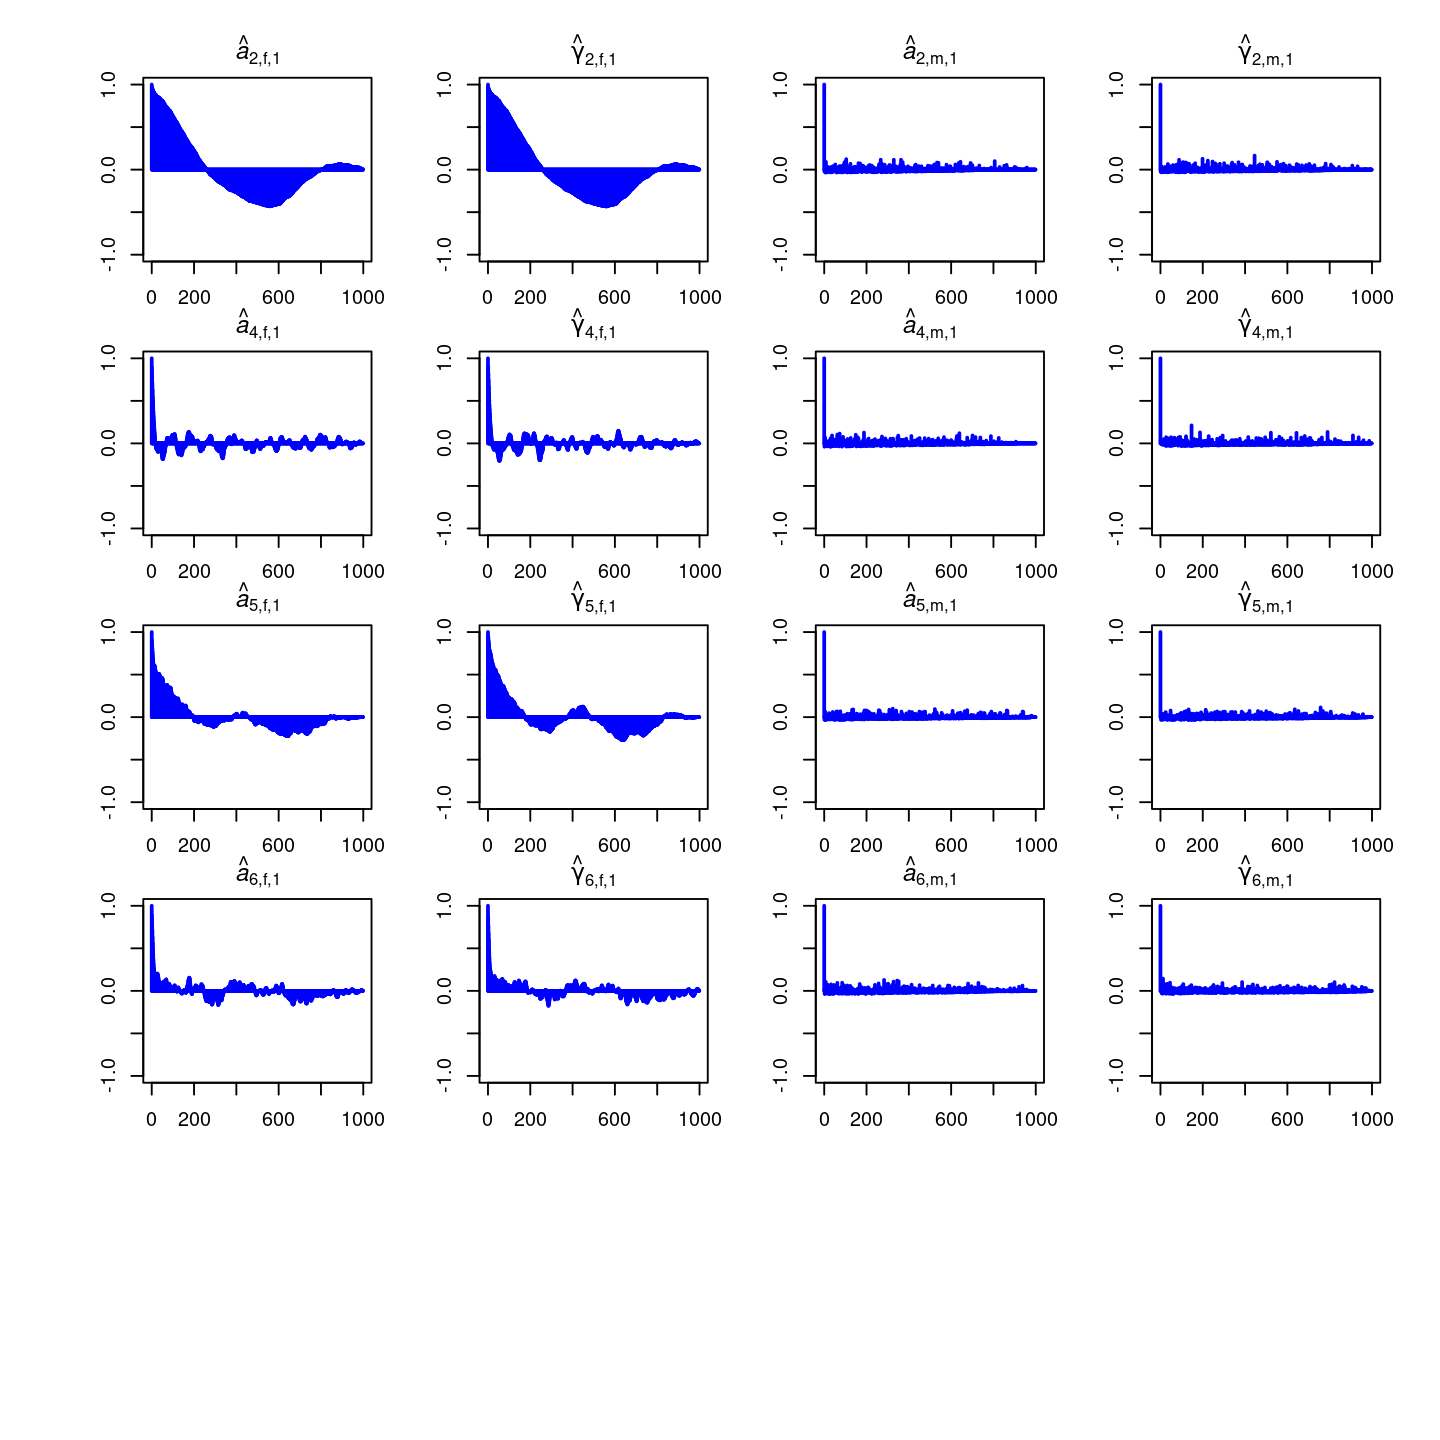
\includegraphics[width=5.5in]{knitr-figs-pdf/fig-base-autocor-selex-1}}{Figure \ref{fig:fig-base-autocor-selex}} 

}

\caption{Autocorrelation plots for MCMC output of estimated selectivity parameters in the base model. The x-axis values are the lag between posteriors. See Figure~\ref{fig:fig-base-trace-selex} for descriptions of the parameter subscripts.}\label{fig:fig-base-autocor-selex}
\end{figure}



\begin{figure}[H]

{\centering \pdftooltip{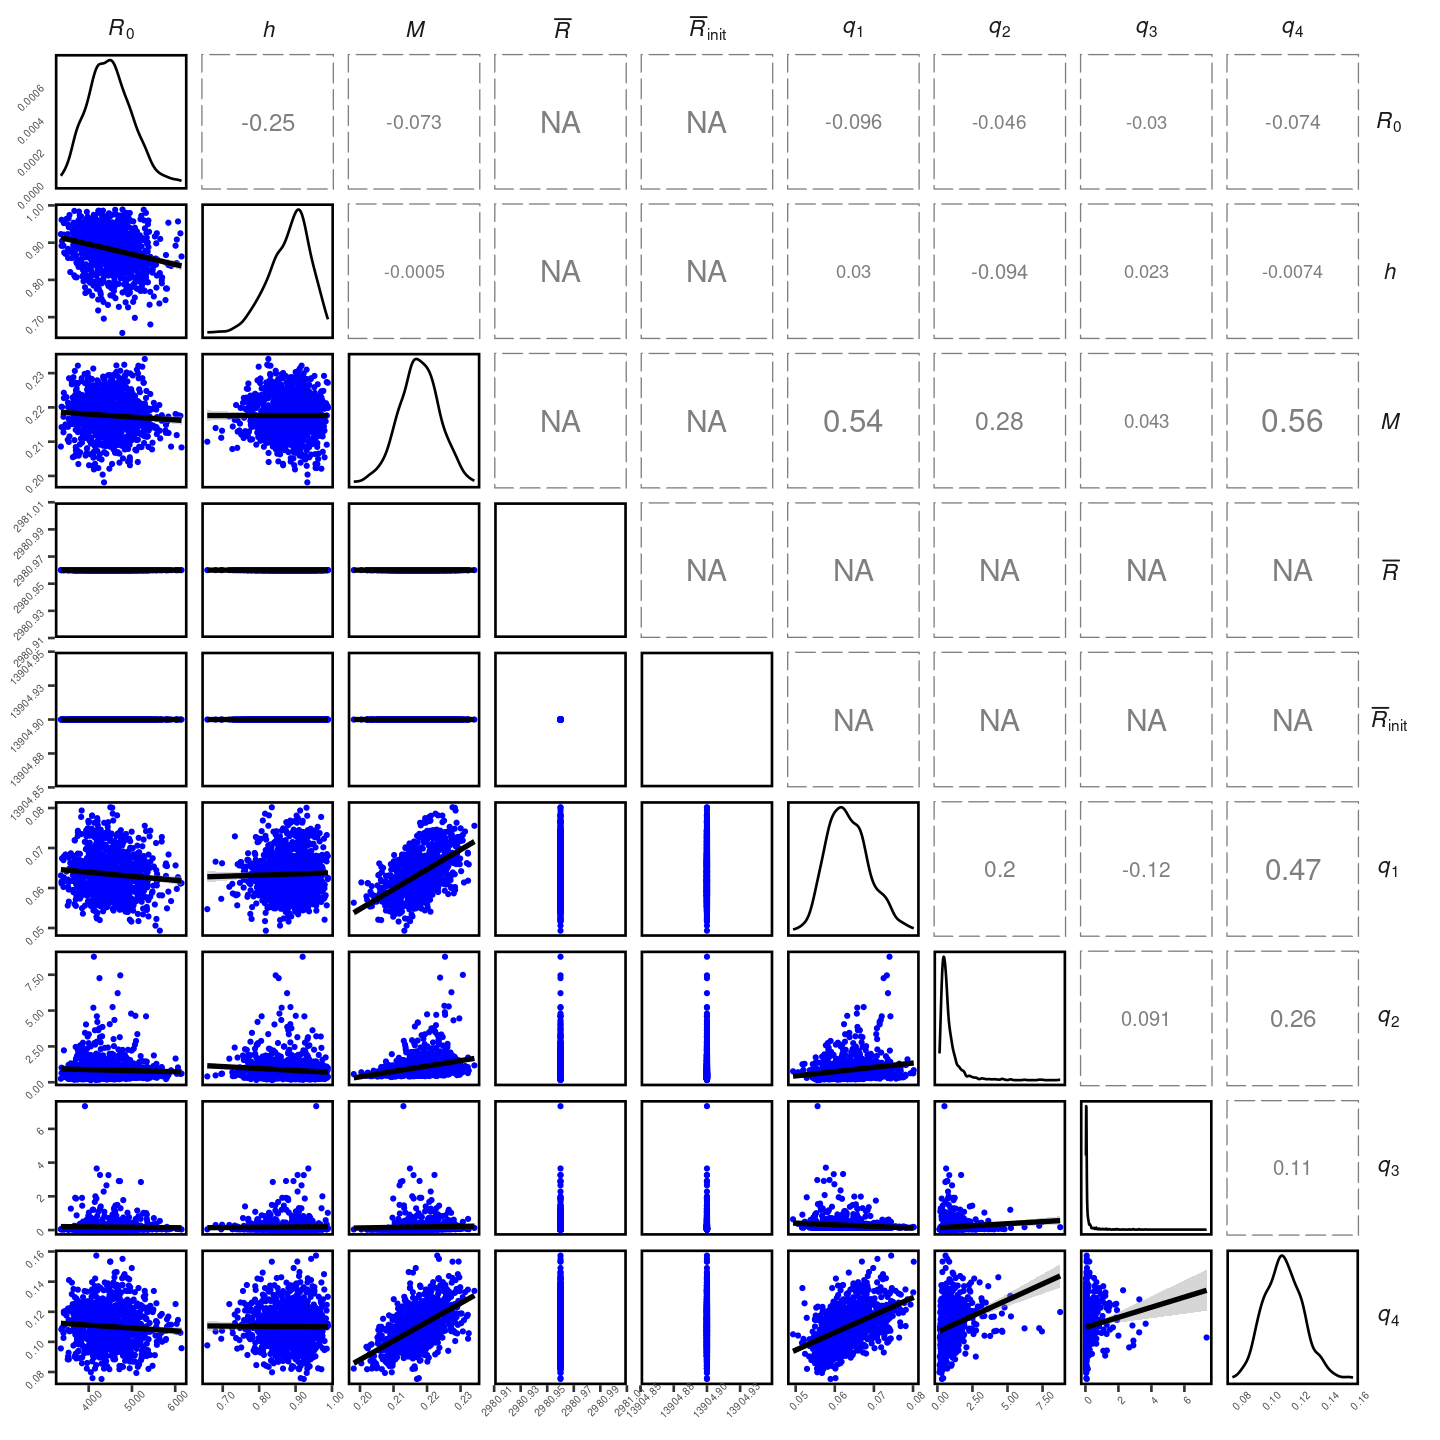
\includegraphics[width=5.5in]{knitr-figs-pdf/fig-base-pairs-1}}{Figure \ref{fig:fig-base-pairs}} 

}

\caption{Pairs plots for MCMC estimated parameters in the base model. The lines in the points plots in the lower triangular panels are linear models with shaded 95\% confidence intervals. The line plots in the diagonal panels represent density of the parameter values, and the values in the upper triangular panels are the correlations between parameters with text size being directly proportional to the absolute value of those values. See Figure~\ref{fig:fig-base-priors-posts} for \(q\) subscript descriptions.}\label{fig:fig-base-pairs}
\end{figure}



\begin{figure}[H]

{\centering \pdftooltip{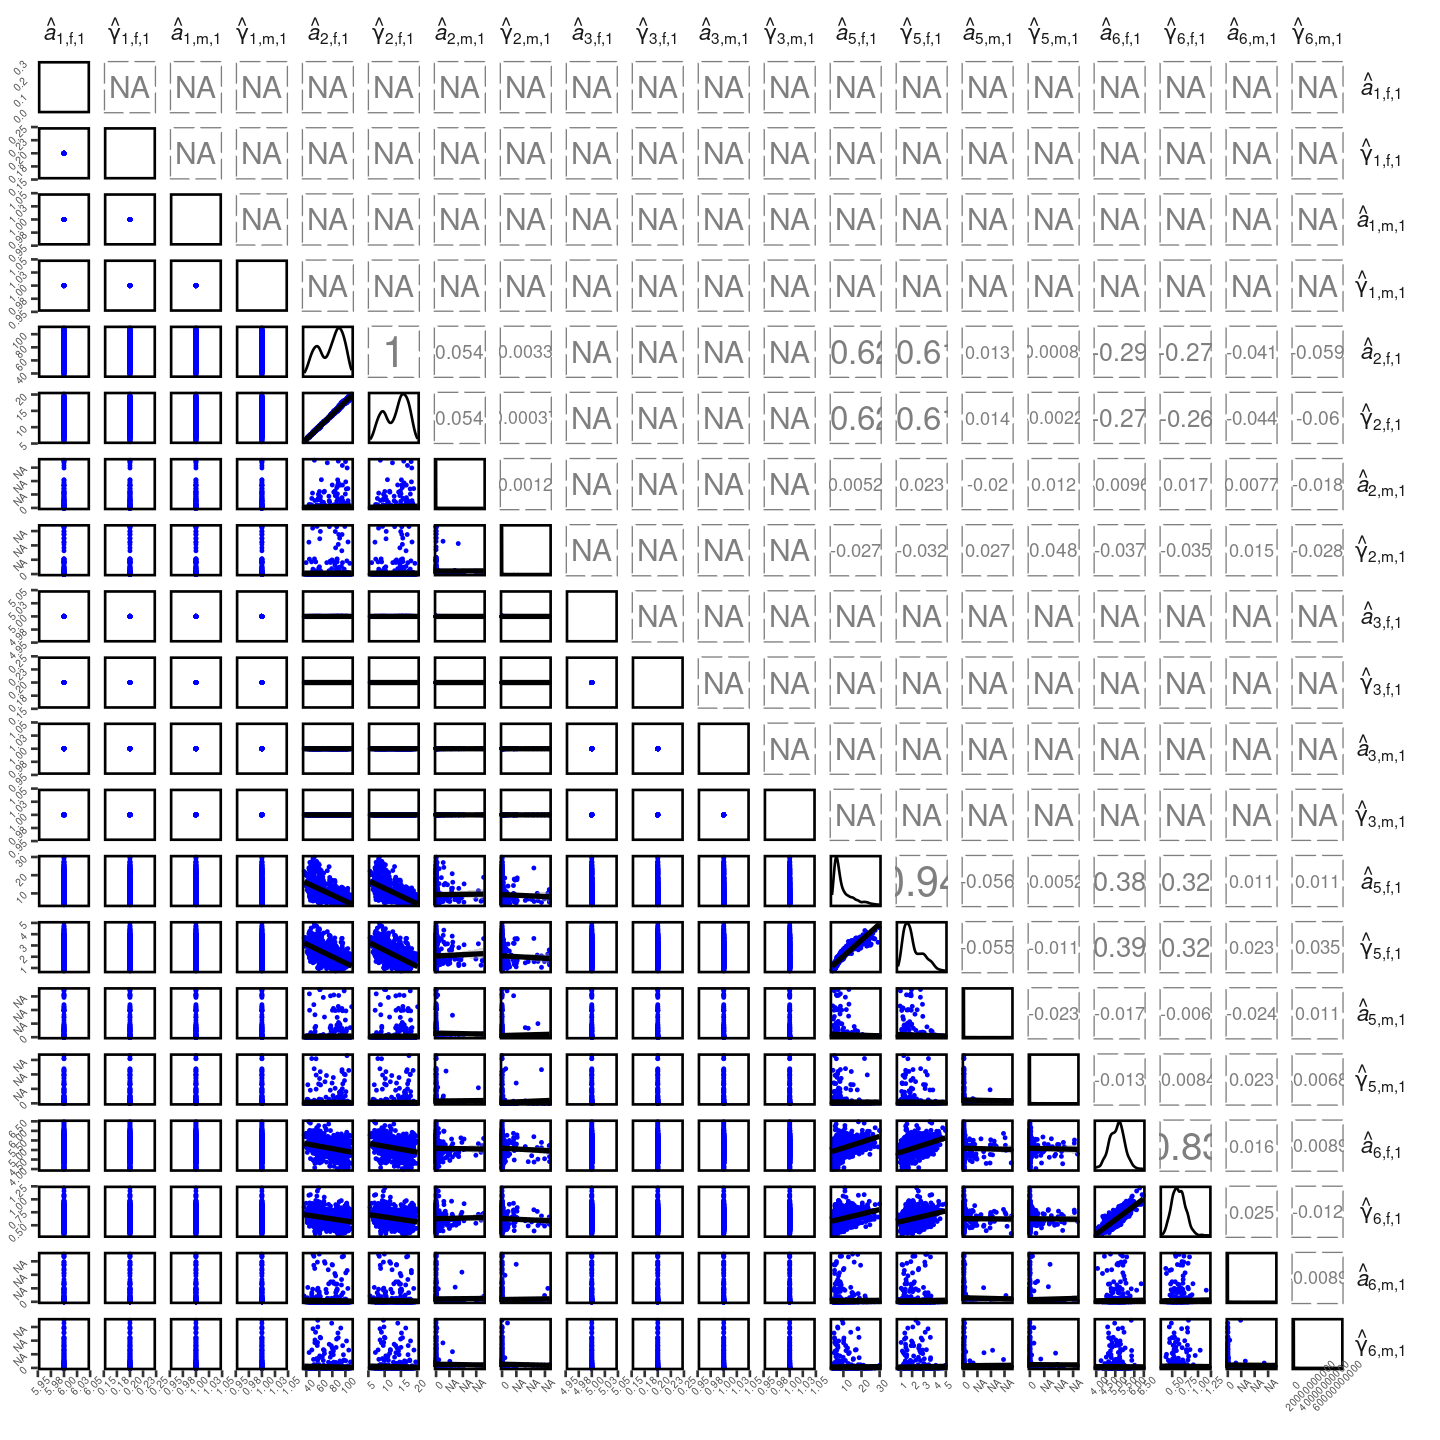
\includegraphics[width=6.5in]{knitr-figs-pdf/fig-base-pairs-sel-1}}{Figure \ref{fig:fig-base-pairs-sel}} 

}

\caption{Pairs plots for MCMC estimated selectivity parameters in the base model. The lines in the points plots in the lower triangular panels are linear models with shaded 95\% confidence intervals. The line plots in the diagonal panels represent density of the parameter values, and the values in the upper triangular panels are the correlations between parameters with text size being directly proportional to the absolute value of those values. See Figure~\ref{fig:fig-base-trace-selex} for descriptions of the parameter subscripts.}\label{fig:fig-base-pairs-sel}
\end{figure}
\clearpage

\hypertarget{sensitivity-model-figures}{%
\subsection{SENSITIVITY MODEL FIGURES}\label{sensitivity-model-figures}}




\begin{figure}[H]

{\centering \pdftooltip{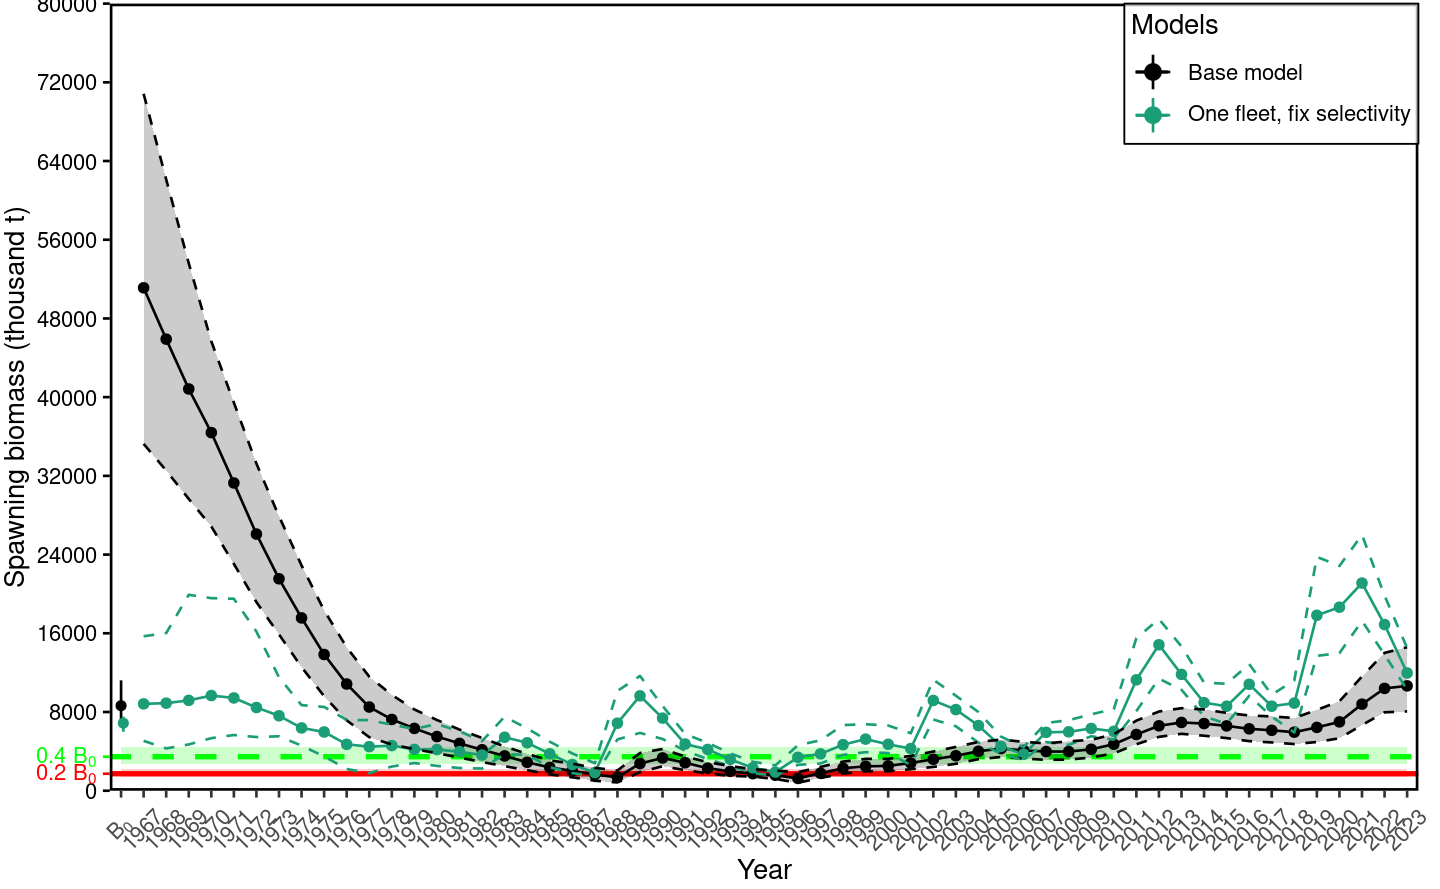
\includegraphics[width=5.5in]{knitr-figs-pdf/fig-sens-variance-1}}{Figure \ref{fig:fig-sens-variance}} 

}

\caption{Spawning biomass for the base model and sensitivity group 1.}\label{fig:fig-sens-variance}
\end{figure}



\begin{figure}[H]

{\centering \pdftooltip{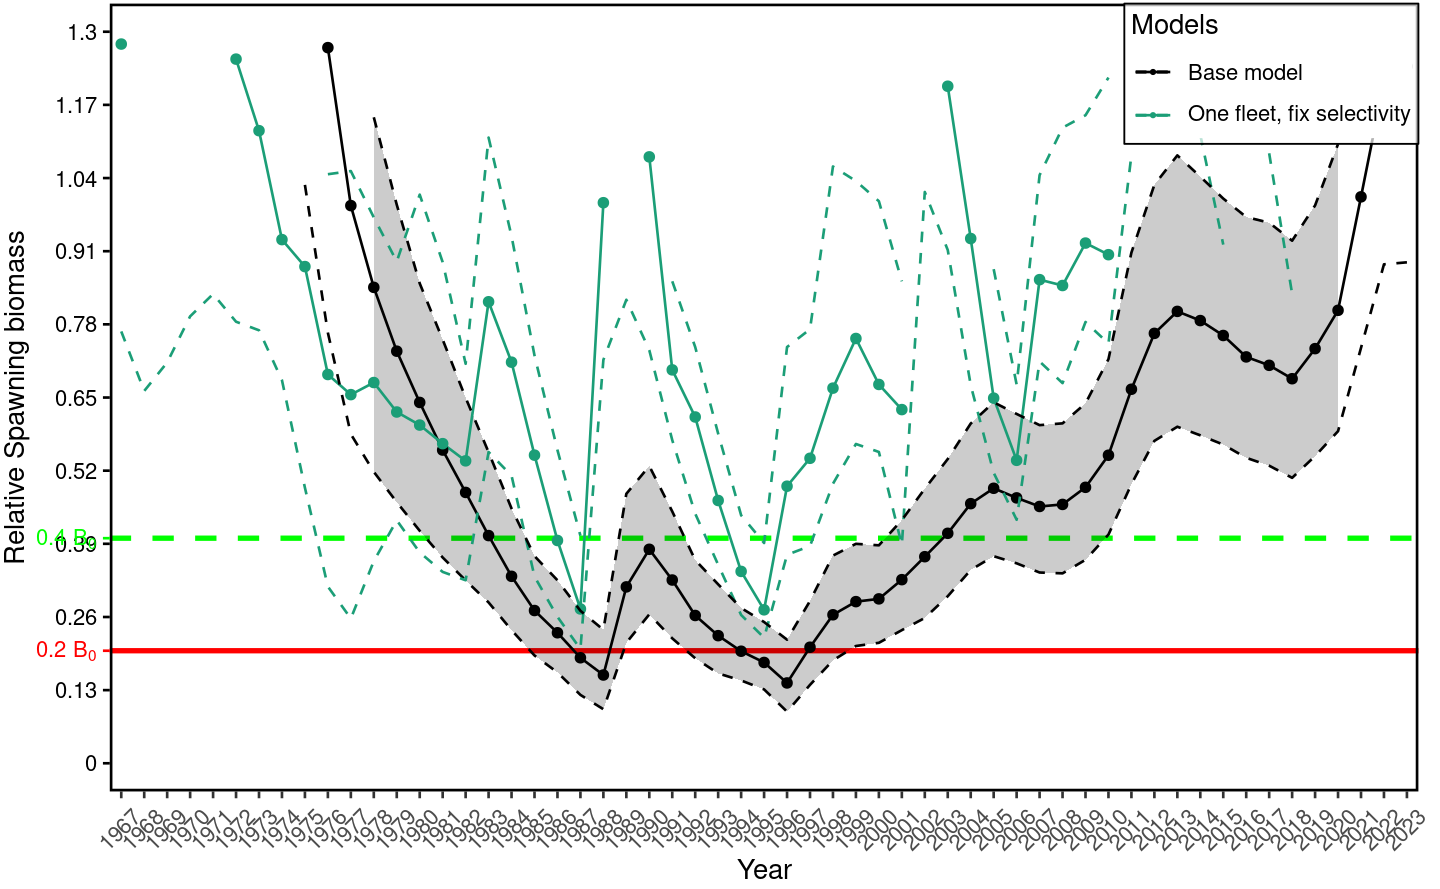
\includegraphics[width=5.5in]{knitr-figs-pdf/fig-sens-variance-rel-1}}{Figure \ref{fig:fig-sens-variance-rel}} 

}

\caption{Relative spawning biomass for the base model and sensitivity group 1.}\label{fig:fig-sens-variance-rel}
\end{figure}



\begin{figure}[H]

{\centering \pdftooltip{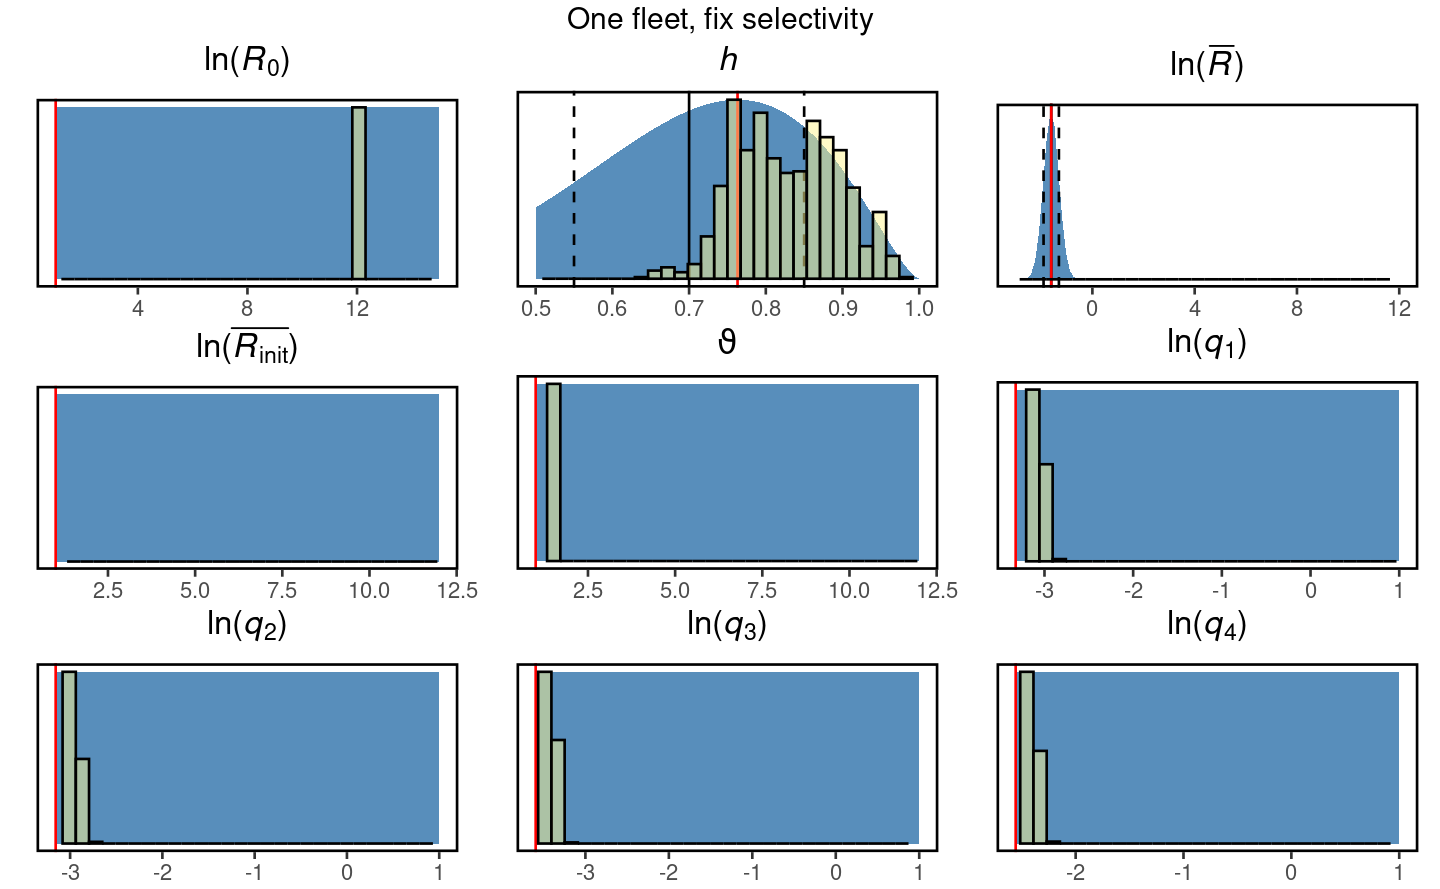
\includegraphics[width=1\linewidth]{knitr-figs-pdf/sens-steepness-prior-1}}{Figure \ref{fig:sens-steepness-prior}} 

}

\caption{Priors and posteriors for the base model and sensitivity model 1.}\label{fig:sens-steepness-prior}
\end{figure}



\begin{figure}[H]

{\centering \pdftooltip{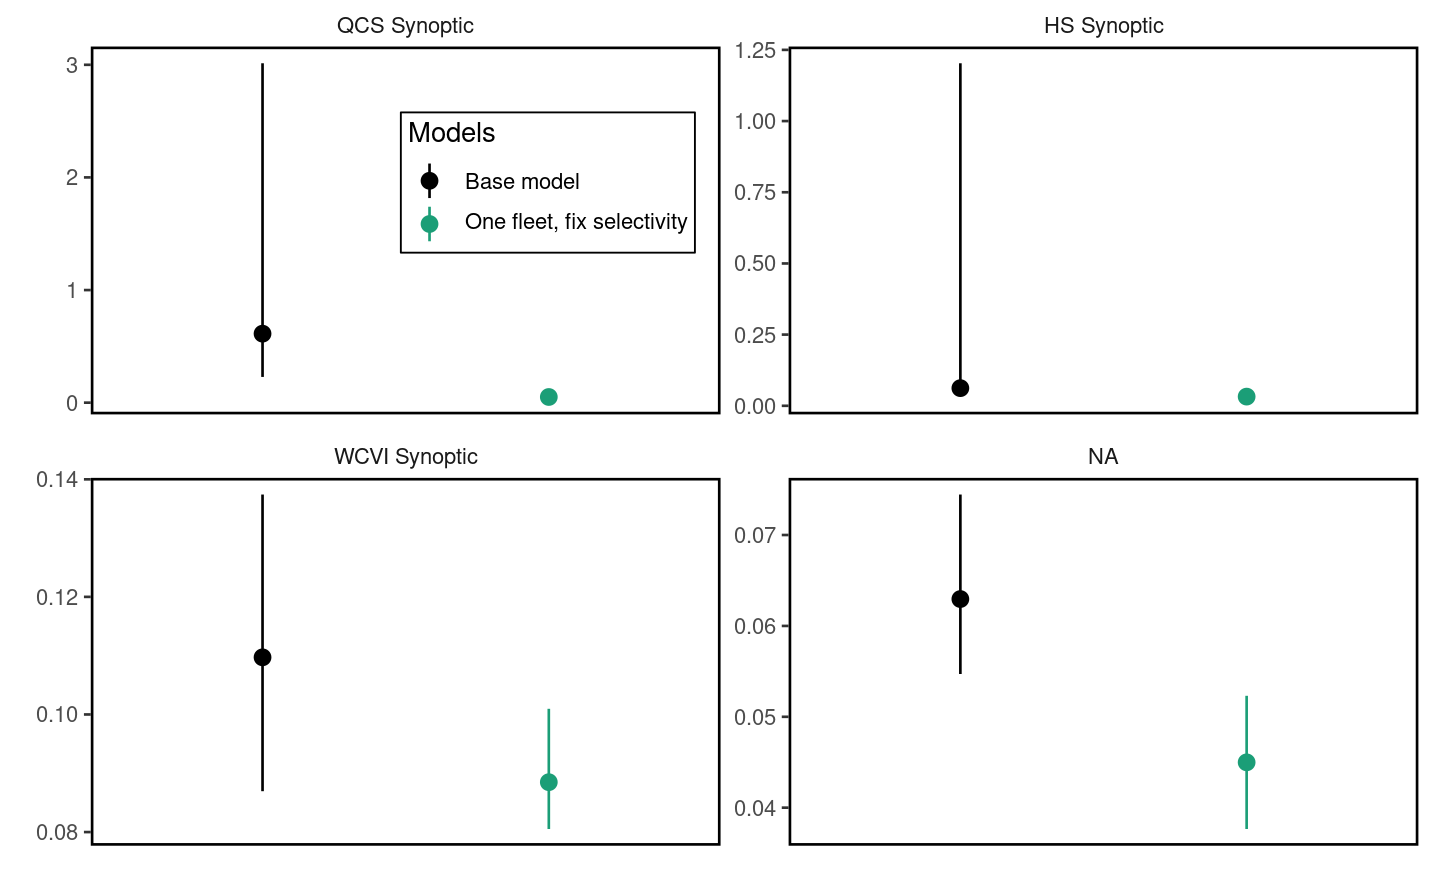
\includegraphics[width=5.5in]{knitr-figs-pdf/fig-sens-q-q-1}}{Figure \ref{fig:fig-sens-q-q}} 

}

\caption{Catchability estimates for the base model and sensitivity group 1.}\label{fig:fig-sens-q-q}
\end{figure}



\begin{figure}[H]

{\centering \pdftooltip{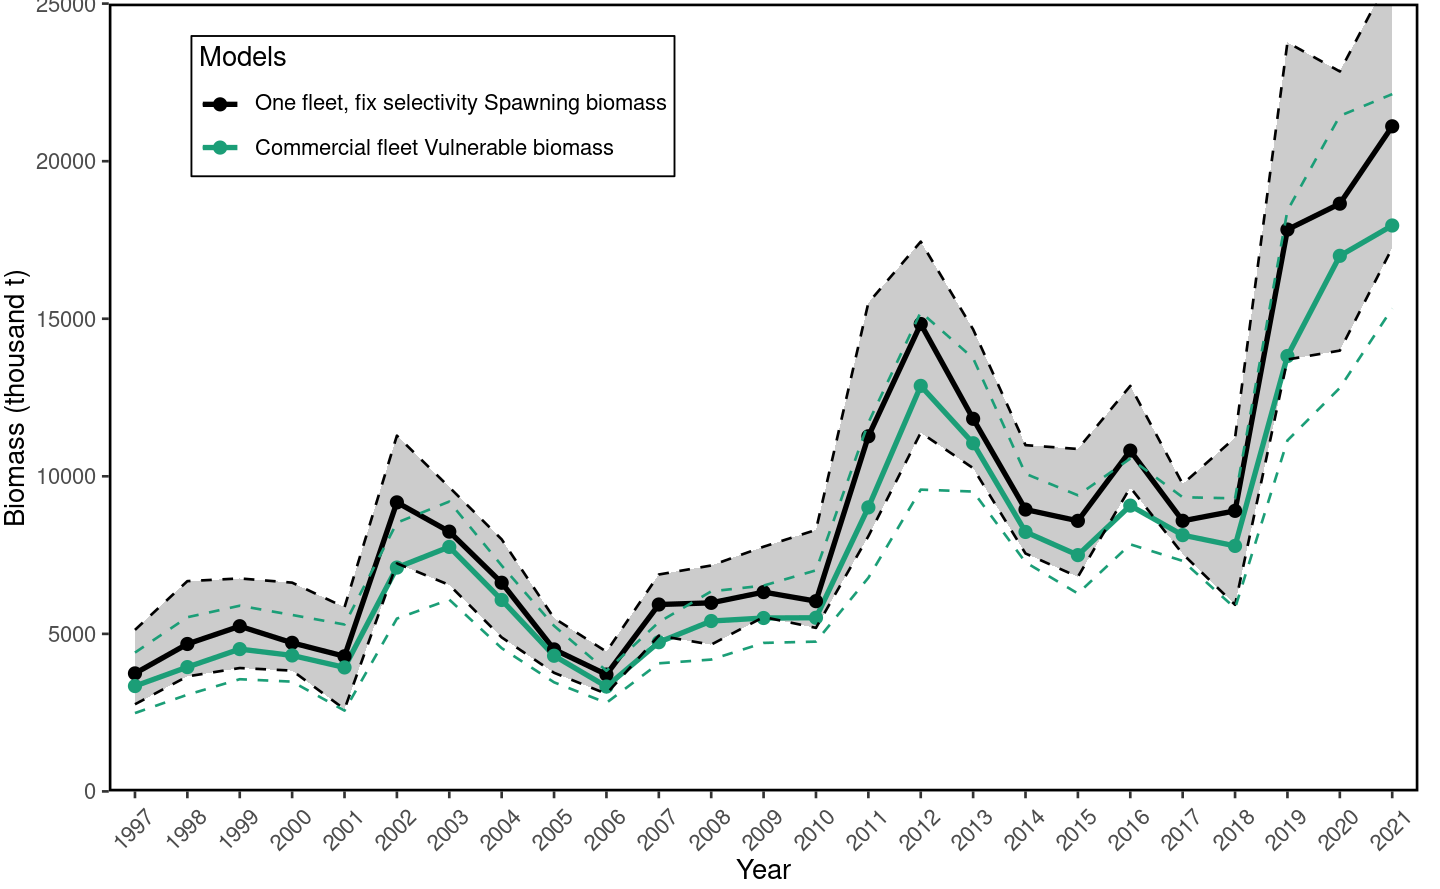
\includegraphics[width=5.5in]{knitr-figs-pdf/fig-sens-sel-eq-mat-vuln-1}}{Figure \ref{fig:fig-sens-sel-eq-mat-vuln}} 

}

\caption{Spawning biomass and vulnerable biomass for the base model and sensitivity group 1.}\label{fig:fig-sens-sel-eq-mat-vuln}
\end{figure}







\begin{figure}[H]

{\centering \pdftooltip{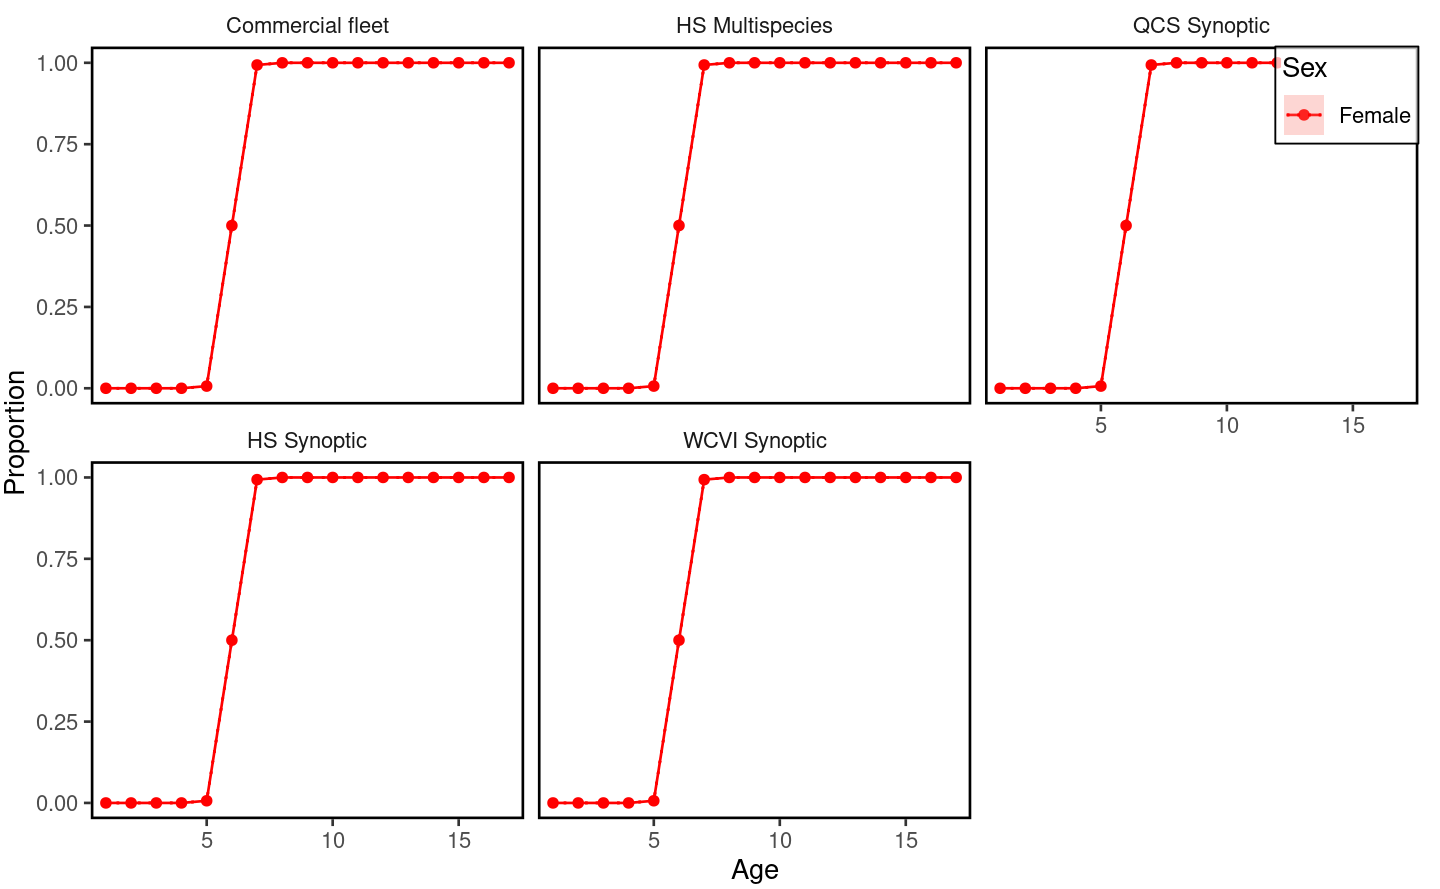
\includegraphics[width=5.5in]{knitr-figs-pdf/fig-sens-qcs-tv-1}}{Figure \ref{fig:fig-sens-qcs-tv}} 

}

\caption{Selectivity for sensitivity group 1.}\label{fig:fig-sens-qcs-tv}
\end{figure}
\clearpage

\clearpage

\hypertarget{references}{%
\section*{REFERENCES}\label{references}}
\addcontentsline{toc}{section}{REFERENCES}

\end{document}
